\chapter{粒子力学、四元动量与静止能量}

\section{我们将反复使用的近似}

相对论性粒子的力学必须用新的语言回答熟悉的问题。粒子如何运动？它的动量和能量是什么？为什么这些量能组合成一个四元矢量，\(E=mc^2\)又是如何从力学的普通机制中涌现出来的？在讨论这些问题之前，我们需要一个初等的近似，它将在整个计算中反复出现。

对任意指数\(p\)，二项级数为
\begin{equation}
\begin{aligned}
(1+\epsilon)^p
&=1+p\epsilon\\
&\quad+\frac{p(p-1)}{2!}\epsilon^2\\
&\quad+\frac{p(p-1)(p-2)}{3!}\epsilon^3
+\cdots .
\end{aligned}
\label{eq:sr3-binomial}
\end{equation}
该指数可以是正数、负数、分数，甚至复数。对于足够小的\(\epsilon\)，级数迅速收敛，且每一项都比前一项更小。于是我们可以在所需精度要求的任意阶处截断。零阶项通常最大，但在下面的应用中它往往是常数，因而在动力学上无趣。运动出现在一阶修正中。

\begin{figure}[htbp]
\centering
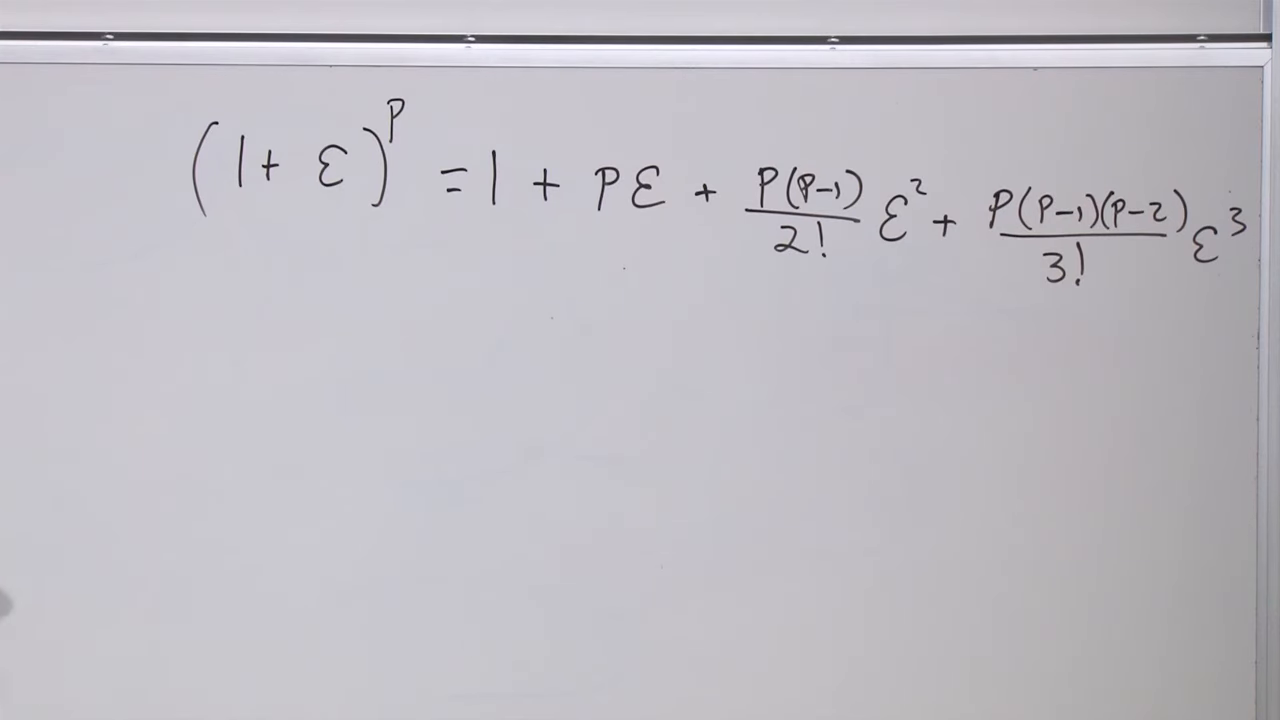
\includegraphics[width=0.90\textwidth]{lecture_03_figure_01.png}
\caption{二项级数展开至三阶，用于从相对论公式恢复非相对论力学。}
\lectureframe{00:04:24}
\end{figure}

我们通常取\(c=1\)，因此速度\(v\)意味着光速的\(v/c\)倍。取\(\epsilon=-v^2\)。当\(p=\tfrac12\)时，
\begin{equation}
\sqrt{1-v^2}
=
1-\frac{v^2}{2}-\frac{v^4}{8}-\cdots
\approx
1-\frac{v^2}{2},
\qquad |v|\ll 1.
\label{eq:sr3-sqrt-expansion}
\end{equation}
当\(p=-\tfrac12\)时，两个负号相消：
\begin{equation}
\frac{1}{\sqrt{1-v^2}}
=
1+\frac{v^2}{2}+\frac{3v^4}{8}+\cdots
\approx
1+\frac{v^2}{2}.
\label{eq:sr3-gamma-expansion}
\end{equation}
经典力学中的许多\(1/2\)因子，事后可以辨认出是这些相对论展开式中一阶修正的结果。当\(v\)趋近于一，该近似失效；此时任何有限截断都无法捕捉精确表达式的奇异行为。

\begin{figure}[htbp]
\centering
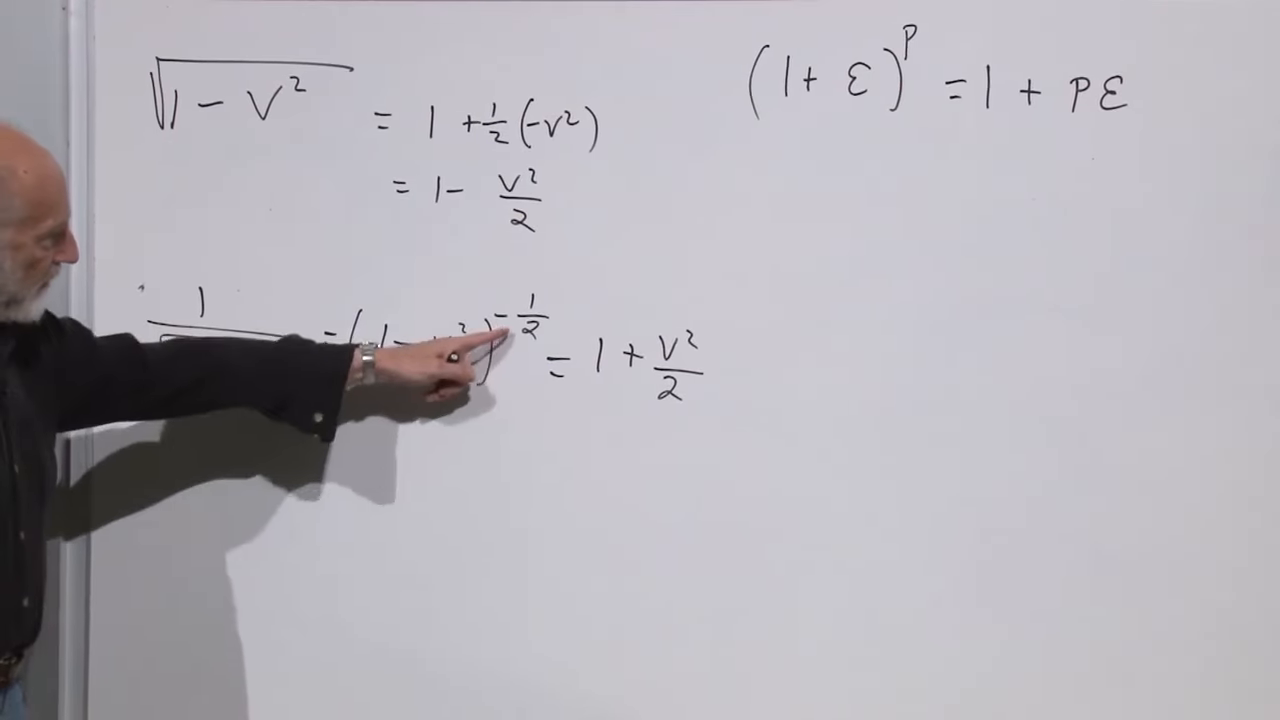
\includegraphics[width=0.90\textwidth]{lecture_03_figure_02.png}
\caption{两个低速公式都可见：\(\sqrt{1-v^2}\approx1-v^2/2\)和\((1-v^2)^{-1/2}\approx1+v^2/2\)。}
\lectureframe{00:07:39}
\end{figure}

\section{什么算作粒子？}

力学中的粒子不必是基本粒子。它可以是电子、太阳、一盒巧克力或一个甜甜圈。重要的是，该物体足够紧密地结合在一起，使其整体运动可以用质心描述。甜甜圈是一个有用的提醒：质心不必位于物质本身之内。

在牛顿力学中，质心变量满足
\begin{equation}
\vec p=m\vec v,
\qquad
K=\frac12mv^2,
\qquad
\vec F=m\vec a.
\label{eq:sr3-newtonian-particle}
\end{equation}
这些公式不关心物体是基本的还是复合的。复合物体还包含内能。例如，一个运动的甜甜圈具有质心动能加上化学能、热能和结合能：
\begin{equation}
E_{\text{Newtonian}}
=
E_{\text{internal}}+\frac12mv^2.
\label{eq:sr3-newtonian-internal}
\end{equation}
内能项与整体质心速度无关。相对论将保留这一区分，但会揭示内能对整体物体的不变质量有贡献。

所需的工具与经典力学中使用的相同：轨迹、稳定作用量原理、拉格朗日量、正则动量、哈密顿量，以及连续对称性与守恒定律之间的关系。

\section{世界线与因果间隔}

将系统的位置水平绘制、时间垂直绘制。它的历史便是时空中的一条曲线。对一个粒子而言，这条曲线就是它的\emph{世界线}。这一概念在牛顿力学中已经存在，但在相对论中它变得基础性，因为洛伦兹变换混合了空间和时间。

考虑两个事件，其间隔为
\begin{equation}
\Delta x^\mu=(\Delta t,\Delta\vec x),
\qquad
\Delta\vec x^{\,2}
=
(\Delta x)^2+(\Delta y)^2+(\Delta z)^2.
\end{equation}
在单位\(c=1\)下，它们的不变间隔为
\begin{equation}
(\Delta\tau)^2
=
(\Delta t)^2-\Delta\vec x^{\,2}.
\label{eq:sr3-interval}
\end{equation}

\subsection{类时间隔}

若\((\Delta t)^2>\Delta\vec x^{\,2}\)，则\((\Delta\tau)^2>0\)，间隔为类时的。存在一个洛伦兹参考系，使这两个事件发生在同一空间点。在该参考系中，连接它们的线是竖直的，时钟可以从一个事件旅行到另一个事件。其经过的读数为固有时\(\Delta\tau\)。

\begin{figure}[htbp]
\centering
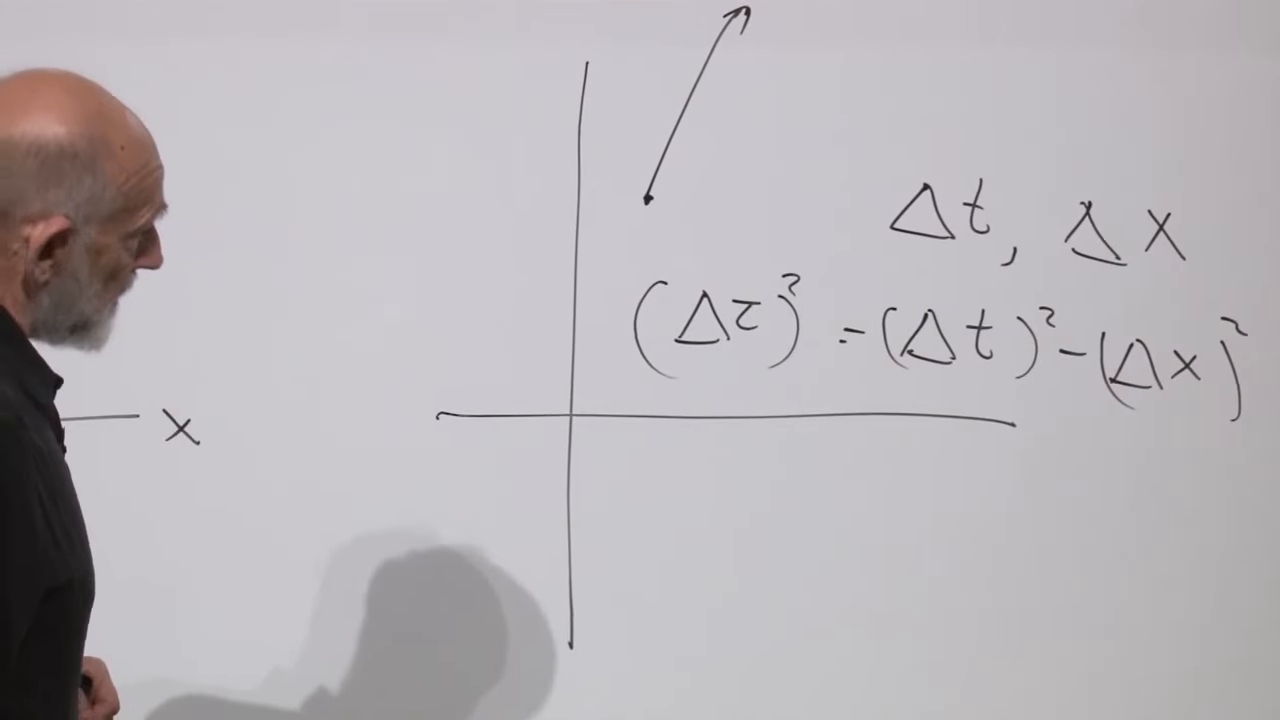
\includegraphics[width=0.90\textwidth]{lecture_03_figure_03.png}
\caption{类时间隔的时间分离大于空间分离；存在一个静止参考系，使两个事件共享同一位置。}
\lectureframe{00:14:42}
\end{figure}

\subsection{类空间隔}

若\(\Delta\vec x^{\,2}>(\Delta t)^2\)，则间隔为类空的。没有任何惯性参考系能使两个事件处于同一空间点，但存在一个参考系使它们同时发生。其他参考系可以颠倒它们的时间顺序。因此，对于类空事件对，\emph{事件\(A\)先发生}和\emph{事件\(B\)先发生}都不是不变陈述。这就是几何形式的同时性相对性。

\begin{figure}[htbp]
\centering
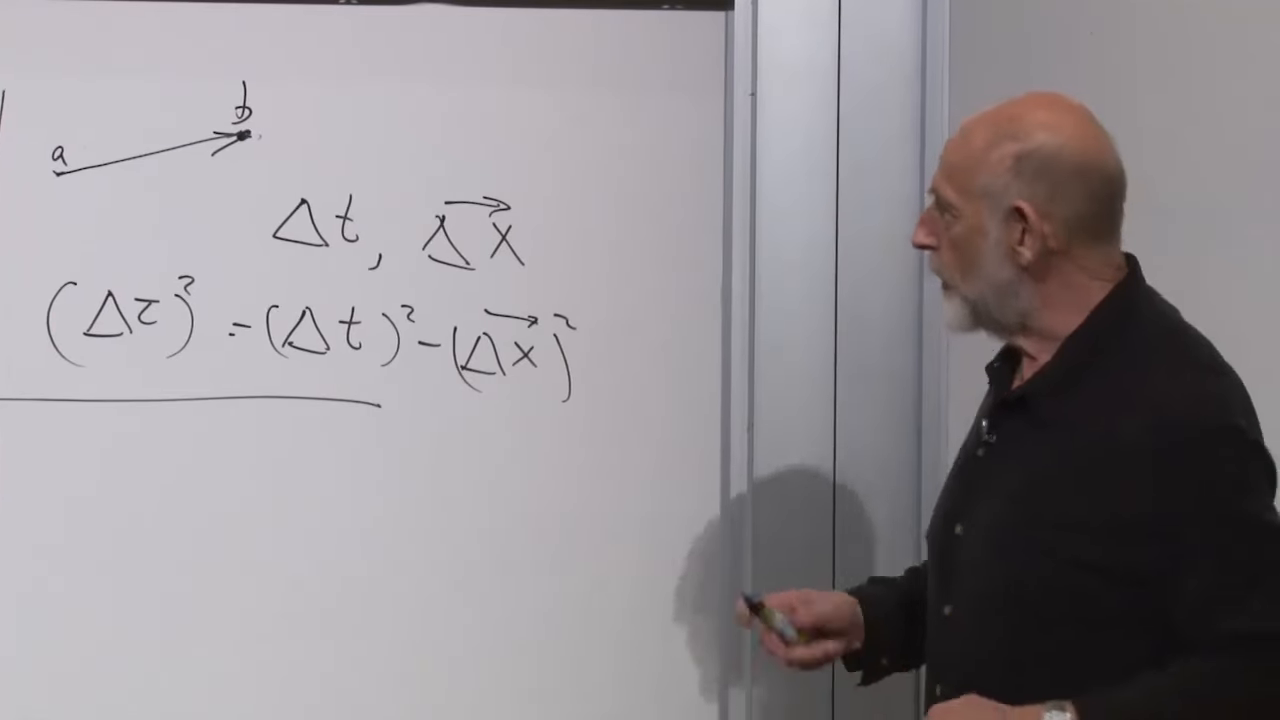
\includegraphics[width=0.90\textwidth]{lecture_03_figure_04.png}
\caption{对于类空间隔，惯性参考系的改变可以使两个事件同时发生或颠倒它们的时间顺序。}
\lectureframe{00:17:01}
\end{figure}

質量を持つ粒子は時間的世界的線を持つ。十分短い任意の線分は\(d\tau^2>0\)を満たす。\(0.9c\)の速度を次々に合成すると、粒子を\(c\)にいくらでも近づけることはできるが、それを超えることは決してない。この接近はゼノンのパラドックスに似ている。この因果的制限は物質的対象だけでなく信号や情報にも当てはまる。情報は物理系によって運ばれなければならないからである。光より速い信号があれば、異なる慣性系がその歴史のどちら端が原因でどちら端が結果かについて一致しなくなるであろう。

\section{四元速度}

短い時間的線分に注目する。従来の単位では、
\begin{equation}
d\tau
=
\sqrt{dt^2-\frac{d\vec x^{\,2}}{c^2}}.
\label{eq:sr3-proper-time-dimensional}
\end{equation}
\(c^2\)の因子は次元によって強制される。\(dt^2\)は時間の二乗の単位を持つのに対し、\(d\vec x^{\,2}\)は長さの二乗の単位を持つからである。

\begin{classroomqa}
\audiencequestion{間隔を通常の単位で書くとき、光速はどこに挿入されなければならないか。}
\lecturerresponse{空間項を\(c^2\)で割らなければならず、\(d\tau^2=dt^2-d\vec x^{\,2}/c^2\)が得られる。通常は\(c=1\)に戻るが、次元の整合性から常に欠けている因子が回復される。\lecturetimestamp{00:21:23}}
\end{classroomqa}

\begin{figure}[htbp]
\centering
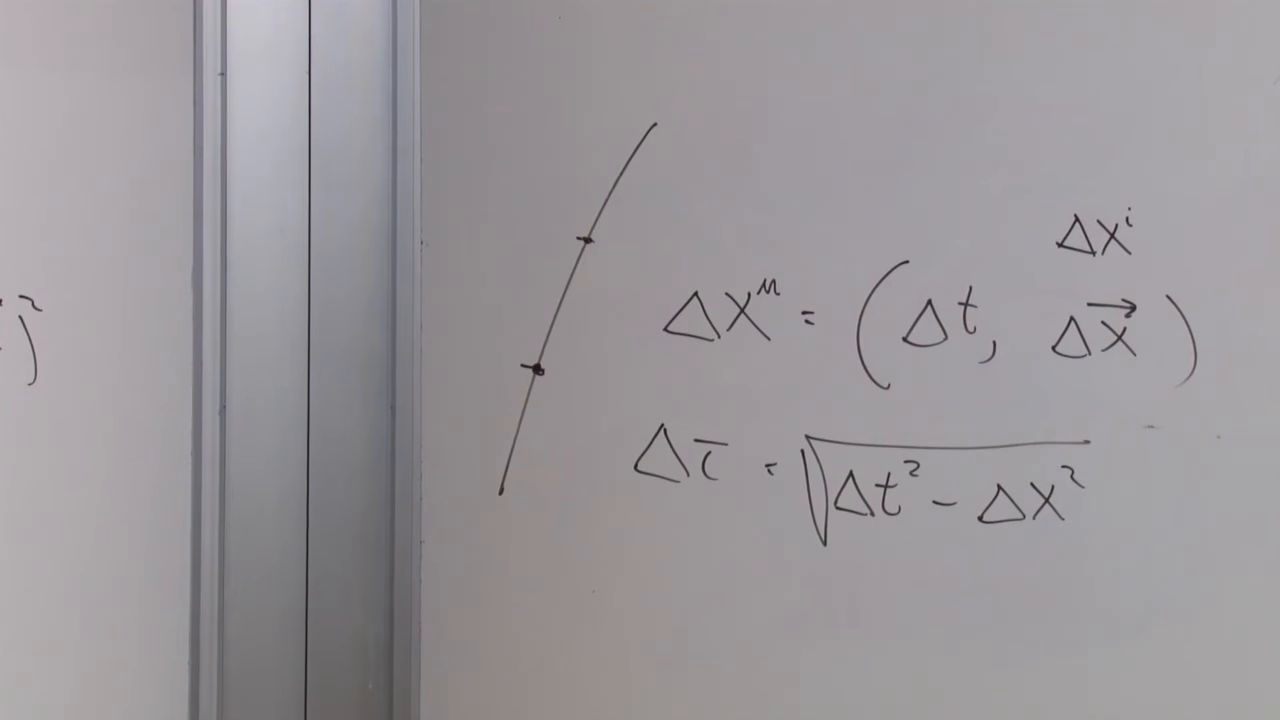
\includegraphics[width=0.90\textwidth]{lecture_03_figure_05.png}
\caption{世界的線の変位\(\Delta x^\mu=(\Delta t,\Delta\vec x)\)とそれに伴う固有時間の増分。}
\lectureframe{00:21:03}
\end{figure}

通常の速度は三つの空間成分を持ち、
\begin{equation}
v^i=\frac{dx^i}{dt},
\qquad i=1,2,3.
\end{equation}
相対論的速度は、完全な時空変位を不変な固有時間で割ることによって得られる：
\begin{equation}
u^\mu
=
\frac{dx^\mu}{d\tau},
\qquad
\mu=0,1,2,3.
\label{eq:sr3-four-velocity-definition}
\end{equation}
ギリシャ文字の添字は時空にわたり、ラテン文字の添字は空間にわたる。位置の第零成分は\(c=1\)単位で\(x^0=t\)であるから、
\begin{equation}
u^0=\frac{dt}{d\tau}.
\end{equation}

\begin{figure}[htbp]
\centering
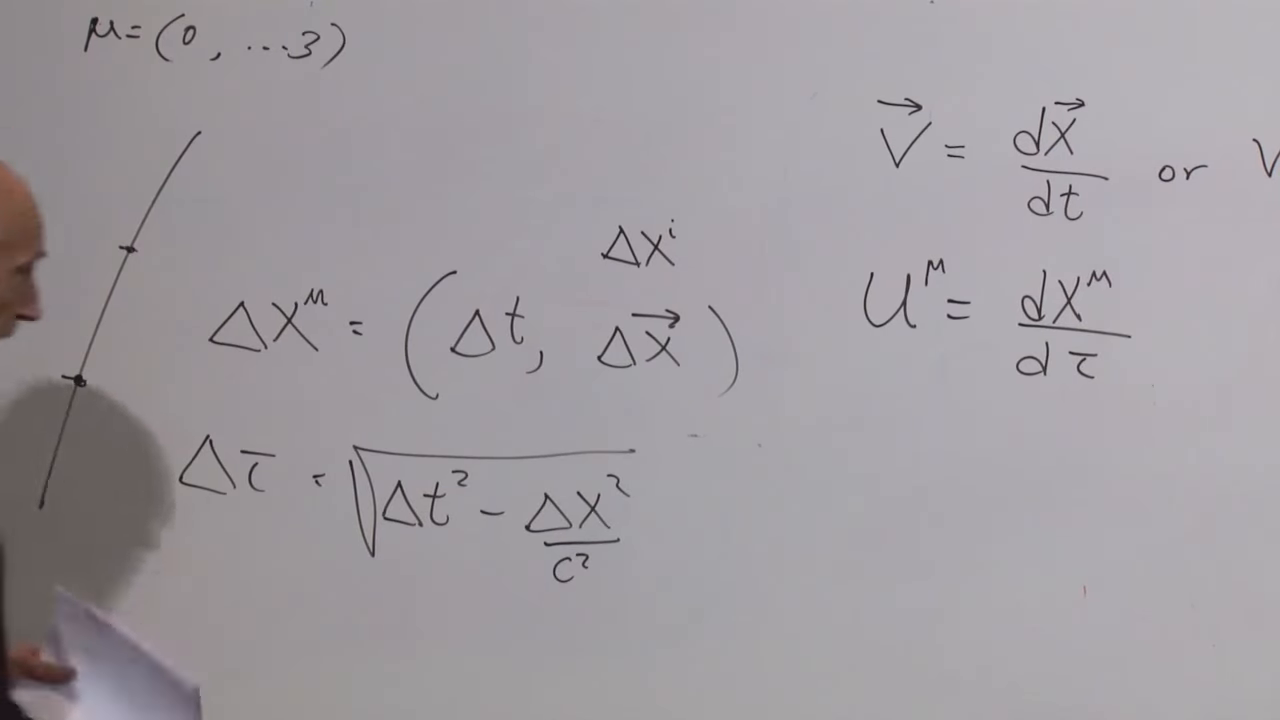
\includegraphics[width=0.90\textwidth]{lecture_03_figure_06.png}
\caption{通常の速度は空間変位を座標時間で割るのに対し、四元速度は四つの成分すべてを固有時間で割る。}
\lectureframe{00:24:05}
\end{figure}

\(u^\mu\)を\(\vec v\)と関係づけるために、間隔から\(dt^2\)をくくり出す：
\begin{align}
d\tau^2
&=dt^2-d\vec x^{\,2}\\
&=dt^2\left(1-\frac{d\vec x^{\,2}}{dt^2}\right)
=dt^2(1-v^2).
\end{align}
未来向きの世界的線に対して正の根を取ると、
\begin{equation}
\frac{d\tau}{dt}=\sqrt{1-v^2},
\qquad
\frac{dt}{d\tau}=\frac{1}{\sqrt{1-v^2}}
\equiv\gamma.
\label{eq:sr3-time-component}
\end{equation}
空間成分については、
\begin{equation}
v^i
=
\frac{dx^i}{dt}
=
\frac{dx^i}{d\tau}\frac{d\tau}{dt}
=u^i\sqrt{1-v^2}.
\end{equation}
したがって
\begin{equation}
\boxed{
u^\mu
=
\gamma(1,\vec v)
},
\qquad
u^0=\gamma,
\qquad
u^i=\gamma v^i.
\label{eq:sr3-four-velocity-components}
\end{equation}
低速では\(u^0\to1\)かつ\(u^i\to v^i\)である。光速近くでは、\(|\vec v|<1\)であっても\(u^0\)と空間的四元速度の大きさの両方が大きくなる。

\begin{figure}[htbp]
\centering
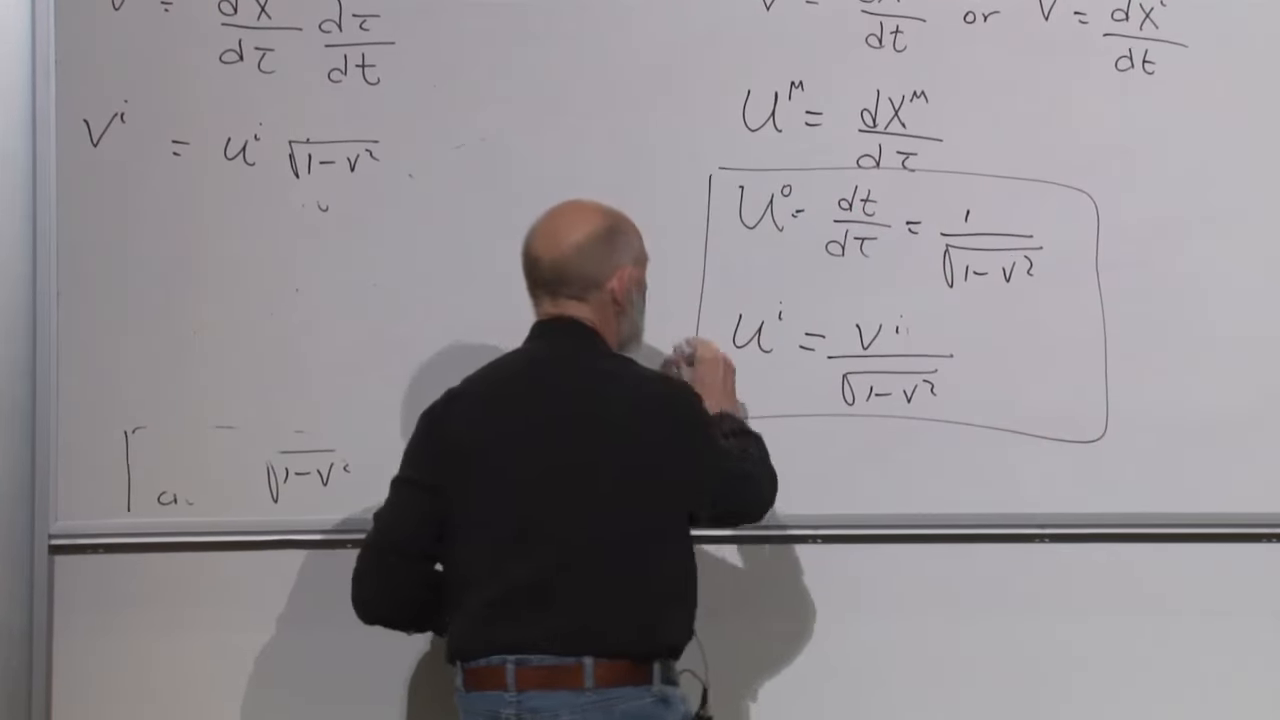
\includegraphics[width=0.90\textwidth]{lecture_03_figure_07.png}
\caption{通常の速度と\(u^\mu\)の四つの成分すべてとの間の確定した関係。}
\lectureframe{00:30:40}
\end{figure}

\subsection{なぜ三つの成分だけが独立なのか}

四元速度は四つの成分を持つが、独立な自由度は三つだけである。間隔の恒等式を\(d\tau^2\)で割ると
\begin{equation}
1
=
\left(\frac{dt}{d\tau}\right)^2
-\left(\frac{d\vec x}{d\tau}\right)^2,
\end{equation}
すなわち
\begin{equation}
\boxed{
(u^0)^2-\vec u^{\,2}=1
}.
\label{eq:sr3-four-velocity-normalization}
\end{equation}
この一つの規格化条件が一つの独立成分を取り除く。

\begin{figure}[htbp]
\centering
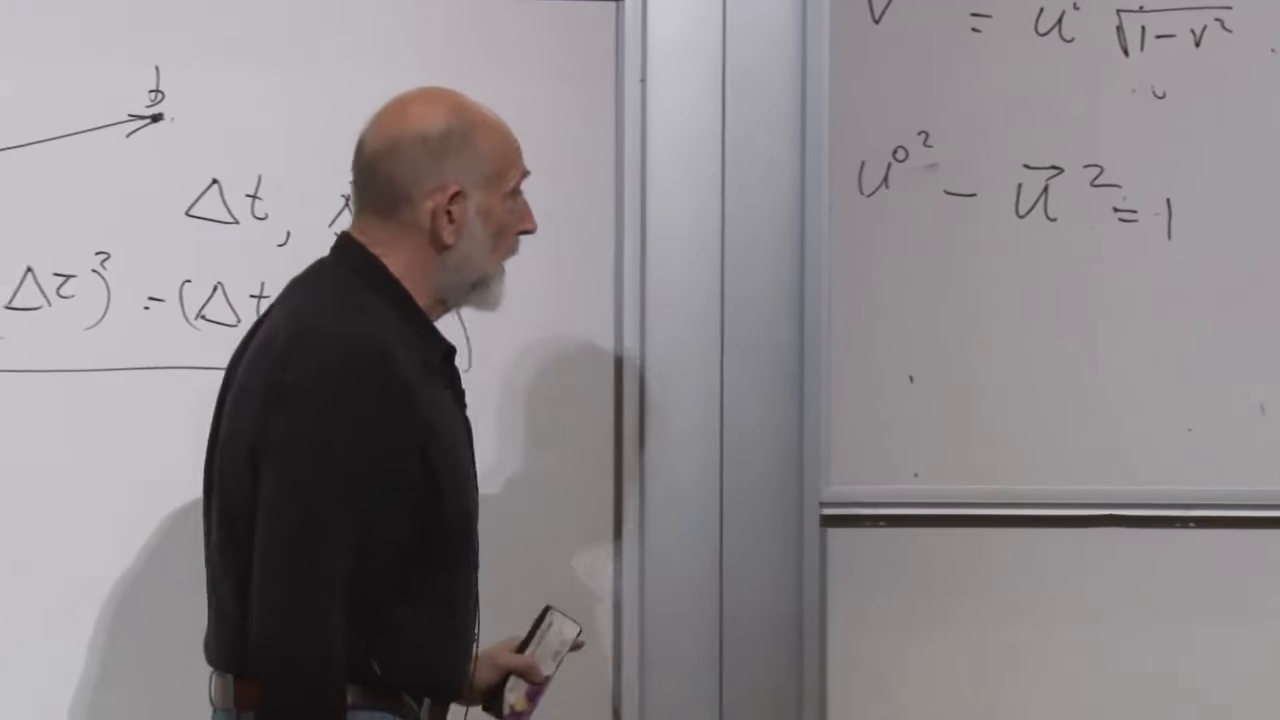
\includegraphics[width=0.90\textwidth]{lecture_03_figure_08.png}
\caption{不変間隔は直ちに規格化\((u^0)^2-\vec u^{\,2}=1\)を与える。}
\lectureframe{00:33:50}
\end{figure}

\begin{classroomqa}
\audiencequestion{一つの独立成分の喪失は、固有時間そのものに関する微分から理解できるか。}
\lecturerresponse{はい。固有時間は独立な第五の座標ではなく、世界的線に沿った時空間隔によって固定される。その定義関係を\(d\tau^2\)で割ると、四つの導関数が単位時間的双曲面\((u^0)^2-\vec u^{\,2}=1\)上にあることが課される。\lecturetimestamp{00:34:07}}
\end{classroomqa}

\section{自由粒子の不変作用}

力を及ぼされない世界的線を支配する法則は何か。古典力学から二つの教訓を保持する：
\begin{enumerate}
\item 物理的経路は、その端点を固定したまま作用を停留にする；
\item 作用は経路の無限小線分から加法的に構成される。
\end{enumerate}
相対性理論は第三の要求を加える：すべての慣性観測者が作用について一致しなければならない。時間的世界的線上で利用できる自然な無限小スカラーは\(d\tau\)である。したがって自由粒子の作用は
\begin{equation}
\boxed{
S=-m\int_a^b d\tau
}
\qquad(c=1).
\label{eq:sr3-invariant-action}
\end{equation}
有限和の描像は
\begin{equation}
S=-m\lim_{N\to\infty}\sum_{k=1}^{N}\Delta\tau_k.
\end{equation}
各固有時間増分についてすべての観測者が一致するので、どの経路がそれらの和を停留にするかについてもすべての観測者が一致する。

\begin{figure}[htbp]
\centering
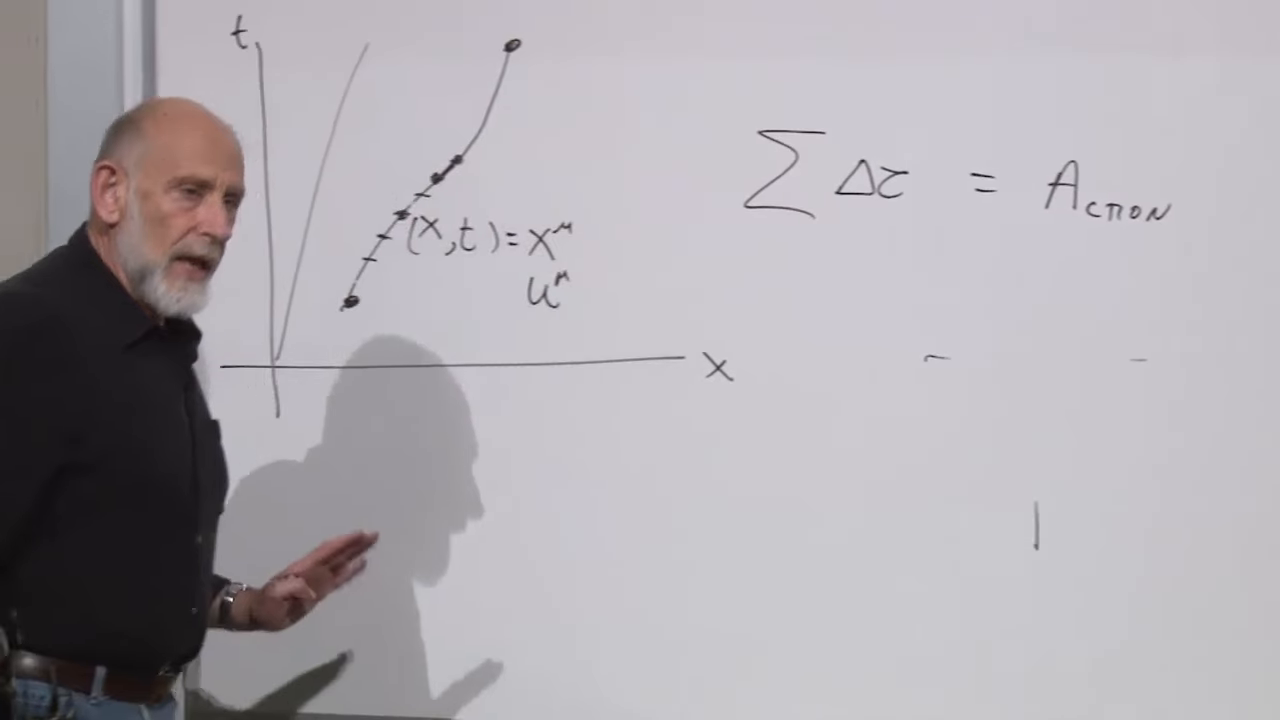
\includegraphics[width=0.90\textwidth]{lecture_03_figure_09.png}
\caption{作用は、端点を固定した変分された世界的線に沿った不変な固有時間増分の和として構成される。}
\lectureframe{00:38:30}
\end{figure}

\begin{classroomqa}
\audiencequestion{作用に任意の定数を掛けるとエネルギーはどうなるか。}
\lecturerresponse{エネルギーは出発点の不変量ではない。それはラグランジアンとハミルトニアンから導かれるであろう。作用全体に非零の定数を掛けてもその停留経路は変わらないが、その作用から定義される正準量は再スケールされる。規格化\(-m\)は、それらの導出量が確立されたニュートン的慣習に一致するように選ばれている。\lecturetimestamp{00:39:47}}
\end{classroomqa}

\begin{classroomqa}
\audiencequestion{固有時のような不変量が、作用を構成するための良い候補となるのはなぜか。}
\lecturerresponse{定常作用の法則は、すべての慣性系で同じ物理的経路を選び出すべきだからである。これはユークリッド平面内で最短曲線を見つけることと類似している。回転は座標成分を変えるが各微小長さは変えないので、どの曲線が最短であるかを変えることはできない。ユークリッド長を固有時で置き換えると、相対論的な構成が得られる。\lecturetimestamp{00:40:39}}
\end{classroomqa}

\begin{classroomqa}
\audiencequestion{固有時に対して負の平方根ではなく正の平方根を選ぶのはなぜか。}
\lecturerresponse{固有時は、過去から未来へ運ばれる時計の正の経過読み取り値として定義される。負の平方根を一貫して選ぶことは、作用の符号を逆にするだけで、最小値を最大値に変えるが、定常な世界線は変わらない。時計の静止系では、正の規約は\(d\tau=dt\)を与える。\lecturetimestamp{00:42:59}}
\end{classroomqa}

因子\(-m\)も同様に、ニュートン力学を再現するために選ばれた規格化の規約である。単位を復元すると、従来の作用は
\begin{equation}
S=-mc^2\int_a^b d\tau.
\label{eq:sr3-action-dimensional}
\end{equation}

\begin{figure}[htbp]
\centering
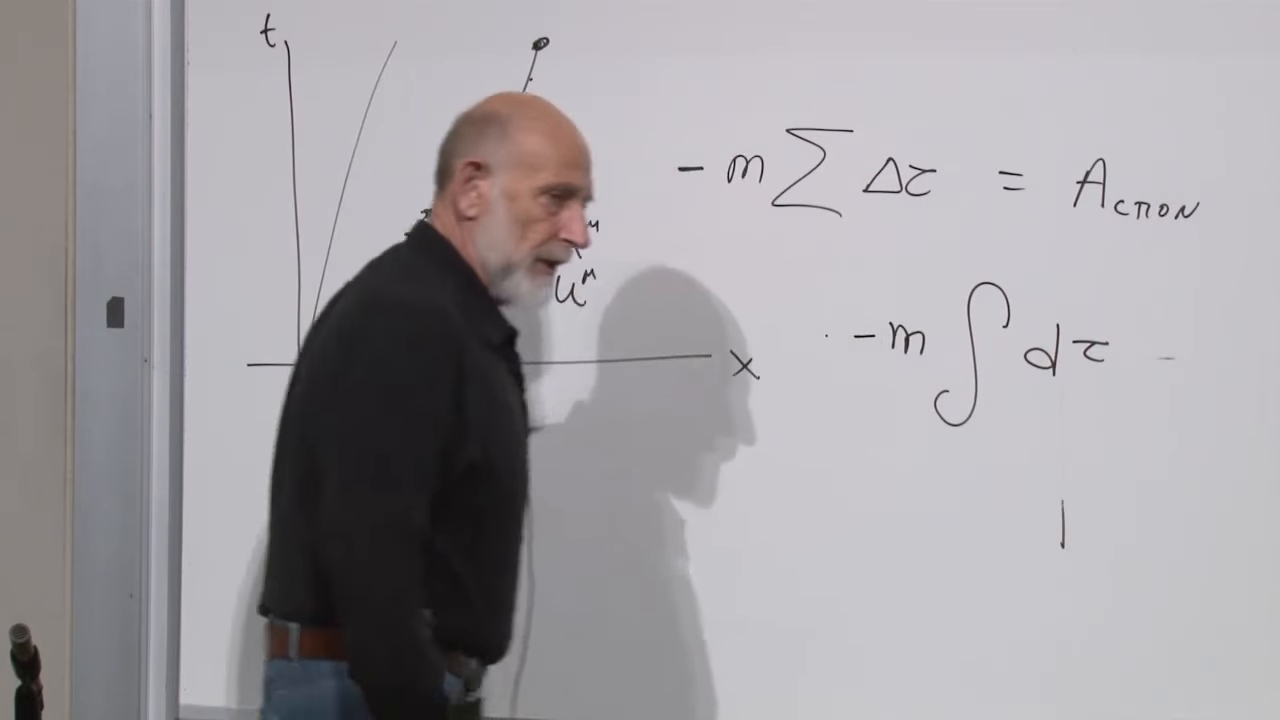
\includegraphics[width=0.90\textwidth]{lecture_03_figure_10.png}
\caption{有限の固有時の和は、自然単位で不変積分\(-m\int d\tau\)になる。}
\lectureframe{00:46:23}
\end{figure}

\section{相対論的ラグランジアン}

作用を標準的な力学の形に置くために、\(d\tau\)から\(dt\)をくくり出す。
\begin{equation}
d\tau
=dt\sqrt{1-\dot{\vec x}^{\,2}},
\qquad
\dot{\vec x}^{\,2}
=\dot x^2+\dot y^2+\dot z^2.
\end{equation}
すると
\begin{equation}
S
=
\int_a^b L\,dt,
\qquad
\boxed{
L=-m\sqrt{1-v^2}
}
\quad(c=1).
\label{eq:sr3-relativistic-lagrangian}
\end{equation}
従来の単位では、
\begin{equation}
L=-mc^2\sqrt{1-\frac{v^2}{c^2}}.
\label{eq:sr3-relativistic-lagrangian-c}
\end{equation}
これは自由粒子のラグランジアンである。速度に依存するが位置には依存しない。力やポテンシャルはまだ導入されていない。

\begin{figure}[htbp]
\centering
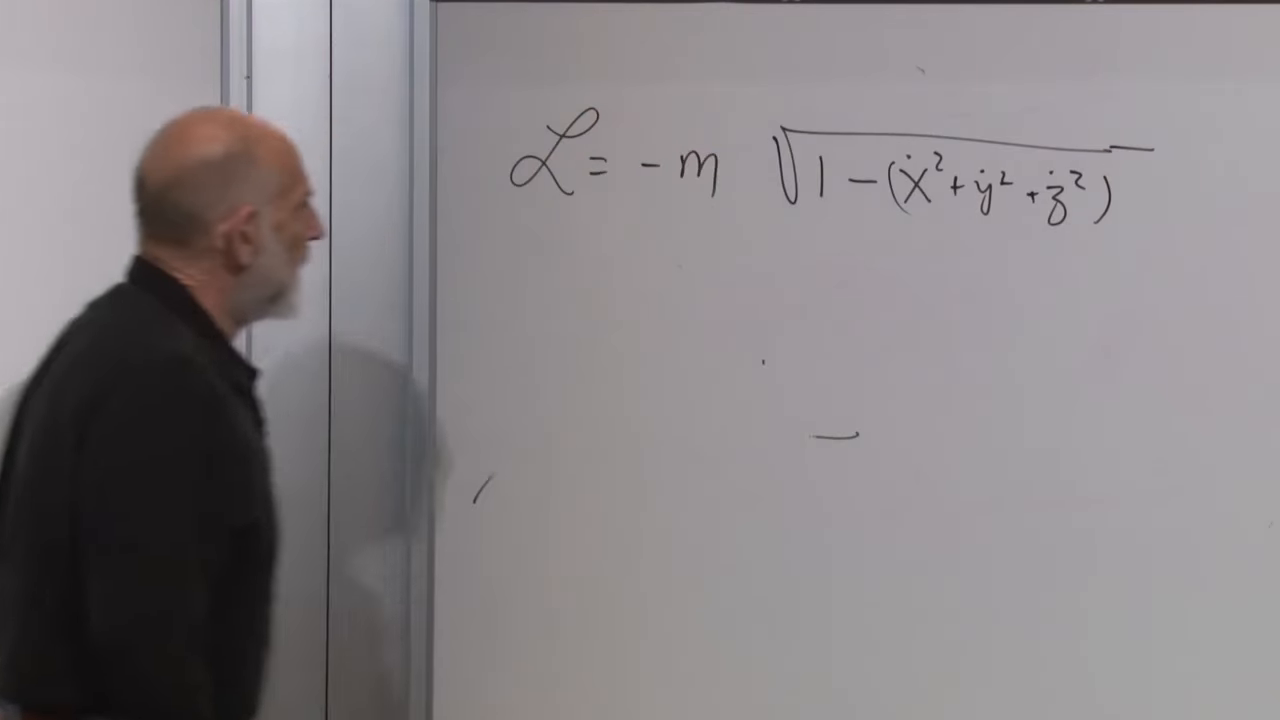
\includegraphics[width=0.90\textwidth]{lecture_03_figure_11.png}
\caption{\(dt\)をくくり出すと、自由相対論的ラグランジアンが3つの速度成分の関数として現れる。}
\lectureframe{00:49:57}
\end{figure}

\subsection{ラグランジュとニュートンの再現}

\eqref{eq:sr3-sqrt-expansion}を代入する。
\begin{align}
L
&=-m\sqrt{1-v^2}\\
&\approx-m\left(1-\frac{v^2}{2}\right)\\
&=-m+\frac12mv^2.
\label{eq:sr3-lagrangian-low-speed}
\end{align}
定数\(-m\)は位置にも速度にも依存しない。同じ端点時刻をもつすべての経路に同じ量を寄与するので、オイラー--ラグランジュ方程式から落ちる。力学的内容をもつ部分はまさに
\begin{equation}
L_{\mathrm{Newton}}=\frac12mv^2.
\end{equation}
したがって、不変作用における符号と質量の規格化は正しく選ばれていた。

\begin{figure}[htbp]
\centering
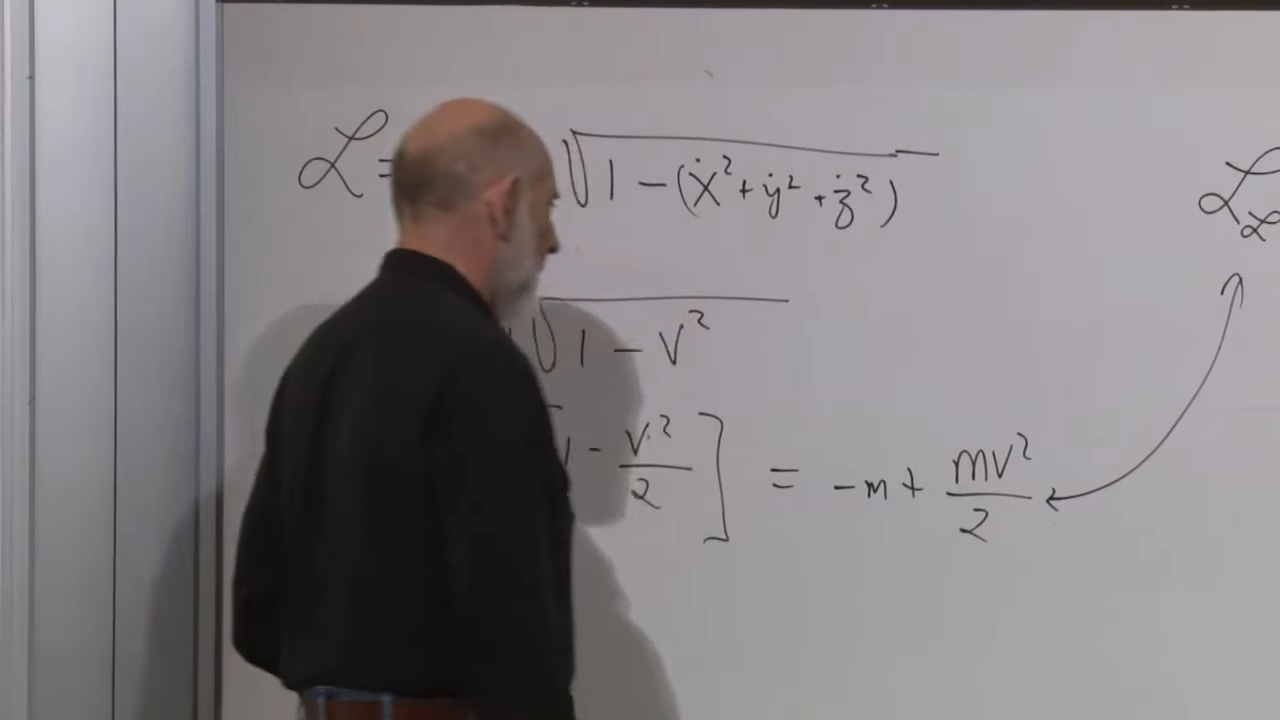
\includegraphics[width=0.90\textwidth]{lecture_03_figure_12.png}
\caption{低速展開は定数\(-m\)とニュートン的自由粒子ラグランジアン\(mv^2/2\)を残す。}
\lectureframe{00:53:24}
\end{figure}

現在の自由粒子に対して、オイラー--ラグランジュ方程式は速度が一定であり時空世界線が直線であることだけを述べる。より明らかにする課題は、保存する運動量とエネルギーを同定することである。

\section{正準運動量}

\(L\)は位置依存性をもたないので、空間並進の下で不変である。対応する保存量は運動量である。ニュートンの公式\(p_i=mv_i\)を仮定するのではなく、正準定義
\begin{equation}
p_i=\frac{\partial L}{\partial\dot x^i}.
\label{eq:sr3-canonical-momentum}
\end{equation}
を用いる。\(L=-m\sqrt{1-v^2}\)に対して、
\begin{align}
p_i
&=
-m\frac{1}{2\sqrt{1-v^2}}
\frac{\partial}{\partial\dot x^i}(1-v^2)\\
&=
-m\frac{1}{2\sqrt{1-v^2}}(-2\dot x^i)\\
&=
\frac{mv_i}{\sqrt{1-v^2}}
=m\gamma v_i.
\label{eq:sr3-relativistic-momentum}
\end{align}
\(u^i=\gamma v^i\)なので、
\begin{equation}
\boxed{
p^i=mu^i
}.
\label{eq:sr3-momentum-spatial}
\end{equation}
低速ではこれは\(p^i\approx mv^i\)に帰着する。光速近くでは分母が決定的に重要になる。

\begin{figure}[htbp]
\centering
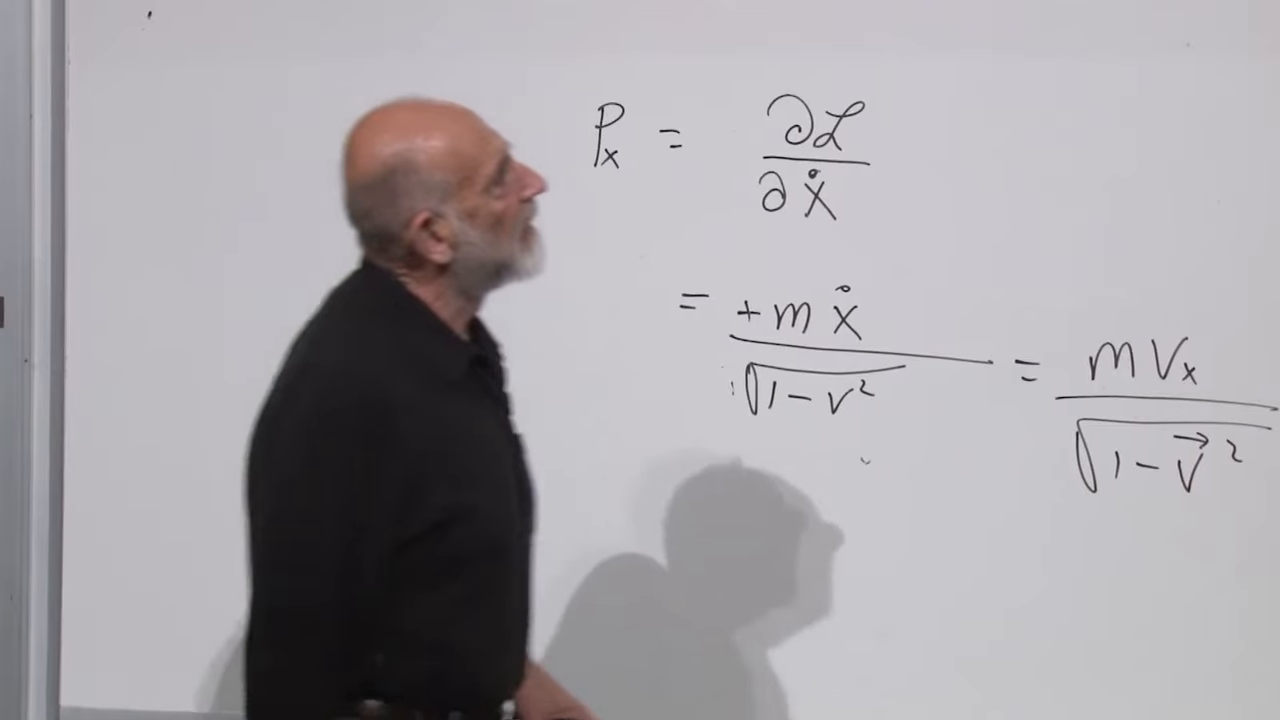
\includegraphics[width=0.90\textwidth]{lecture_03_figure_13.png}
\caption{平方根ラグランジアンの正準的微分は\(p_x=mv_x/\sqrt{1-v^2}\)を与える。}
\lectureframe{00:58:49}
\end{figure}

\subsection{質量であり、相対論的質量ではない}

ここで\(m\)は単に粒子の質量である。粒子が運動しても変化しない不変なラベルである。古い教科書ではこれを\emph{静止質量}と呼び、\(E/c^2\)を速度依存の\emph{相対論的質量}と呼ぶことがある。現代の用法ではその分割を避ける。運動が変えるのはエネルギーと運動量であり、不変質量ではない。電子の質量はどの系でも同じパラメータである。

\section{3元運動量から4元運動量へ}

4元ベクトルの1つの成分についての言明は、一般に系に依存する。たとえば\(\Delta\vec x=0\)は、2つの事象がある系で同じ位置を共有することを述べるが、ブーストはその間隔を傾け、\(\Delta\vec x'\ne0\)とする。対照的に、
\begin{equation}
\Delta x^\mu=0
\end{equation}
は不変である。もし4つの成分すべてがある系で消えるなら、4つすべてがどの系でも消える。同様に、\(\vec u=0\)は粒子の静止系を同定するだけであり、4元速度の不変な記述ではない。

閉じた系に対して、通常の運動量保存は
\begin{equation}
\vec P_{\mathrm{initial}}-\vec P_{\mathrm{final}}=0.
\label{eq:sr3-three-momentum-conservation}
\end{equation}
と書ける。これは3元ベクトル方程式である。保存を明白にローレンツ共変にするには、3つの\(p^i=mu^i\)に加わる第4の成分が必要である。明らかな完成は
\begin{equation}
p^\mu=mu^\mu.
\label{eq:sr3-four-momentum}
\end{equation}
である。\(c=1\)単位では、
\begin{equation}
p^\mu=(p^0,\vec p)
=
m\gamma(1,\vec v).
\end{equation}

\begin{figure}[htbp]
\centering
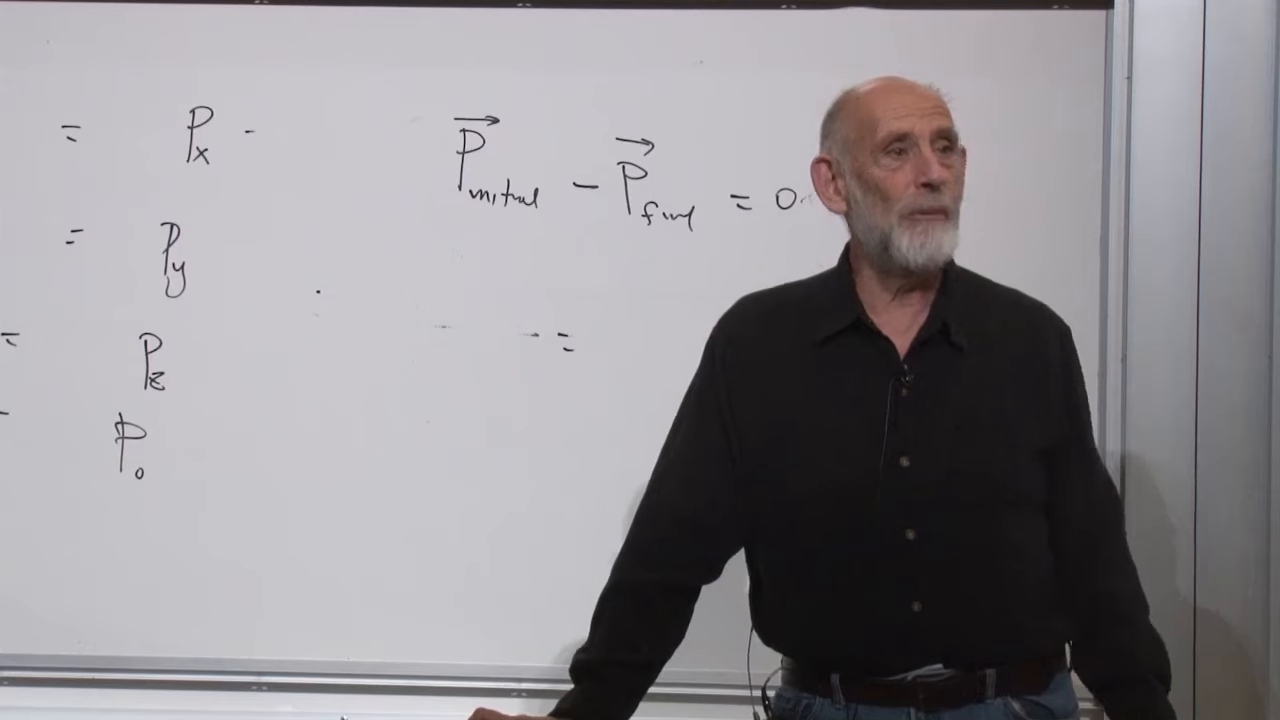
\includegraphics[width=0.90\textwidth]{lecture_03_figure_14.png}
\caption{運動量保存は、空間成分が第4の成分によって完成されて初めて不変になる。}
\lectureframe{01:09:51}
\end{figure}

欠けている成分それ自体も保存されなければならない。粒子力学にはすでに別の保存量が含まれている。すなわちエネルギーである。問題は、\(p^0=mu^0=m\gamma\) が自然単位でまさにそのエネルギーであるかどうかである。体系的な答えはハミルトニアンから得られる。

\section{ハミルトニアンはエネルギーである}

この形の任意の時間に依存しないラグランジアンに対して、ハミルトニアンは
\begin{equation}
H=\sum_{i=1}^{3}\dot x^i p_i-L.
\label{eq:sr3-hamiltonian-definition}
\end{equation}
である。この式は特にニュートン力学に固有のものではない。これは速度から正準運動量への一般的なルジャンドル変換であり、相対論的ラグランジアンにも等しく適用される。

\begin{figure}[htbp]
\centering
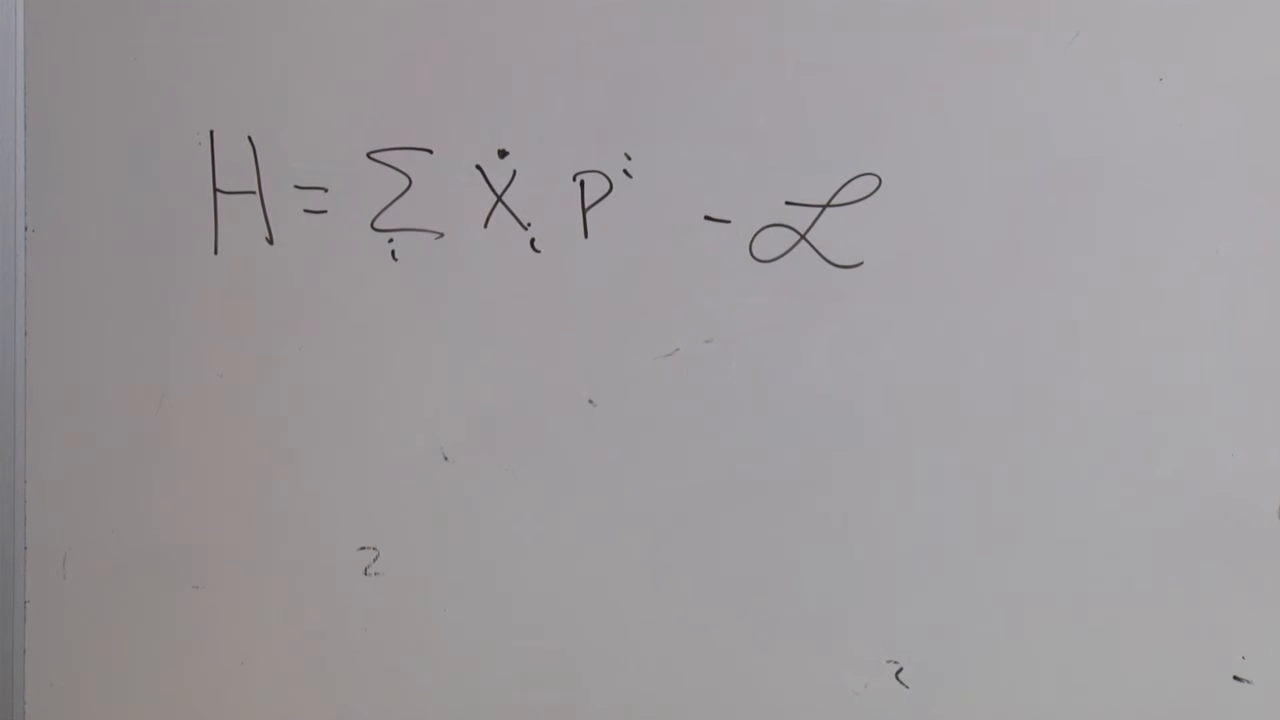
\includegraphics[width=0.90\textwidth]{lecture_03_figure_15.png}
\caption{一般的なハミルトニアンの式 \(H=\sum_i\dot x^i p_i-L\)。}
\lectureframe{01:11:55}
\end{figure}

\(p_i=m\dot x_i/\sqrt{1-v^2}\) と \(L=-m\sqrt{1-v^2}\) を代入すると、
\begin{align}
H
&=
\frac{mv^2}{\sqrt{1-v^2}}
+m\sqrt{1-v^2}\\
&=
\frac{mv^2+m(1-v^2)}{\sqrt{1-v^2}}\\
&=
\boxed{\frac{m}{\sqrt{1-v^2}}}
=m\gamma.
\label{eq:sr3-hamiltonian-result}
\end{align}
この相殺が鍵となる段階である。\(u^0=\gamma\) と比較すると、
\begin{equation}
H=mu^0=p^0.
\end{equation}
したがって第4成分はエネルギーである。
\begin{equation}
p^\mu=(E,\vec p),
\qquad
E=H
\qquad(c=1).
\label{eq:sr3-four-momentum-natural}
\end{equation}

\begin{figure}[htbp]
\centering
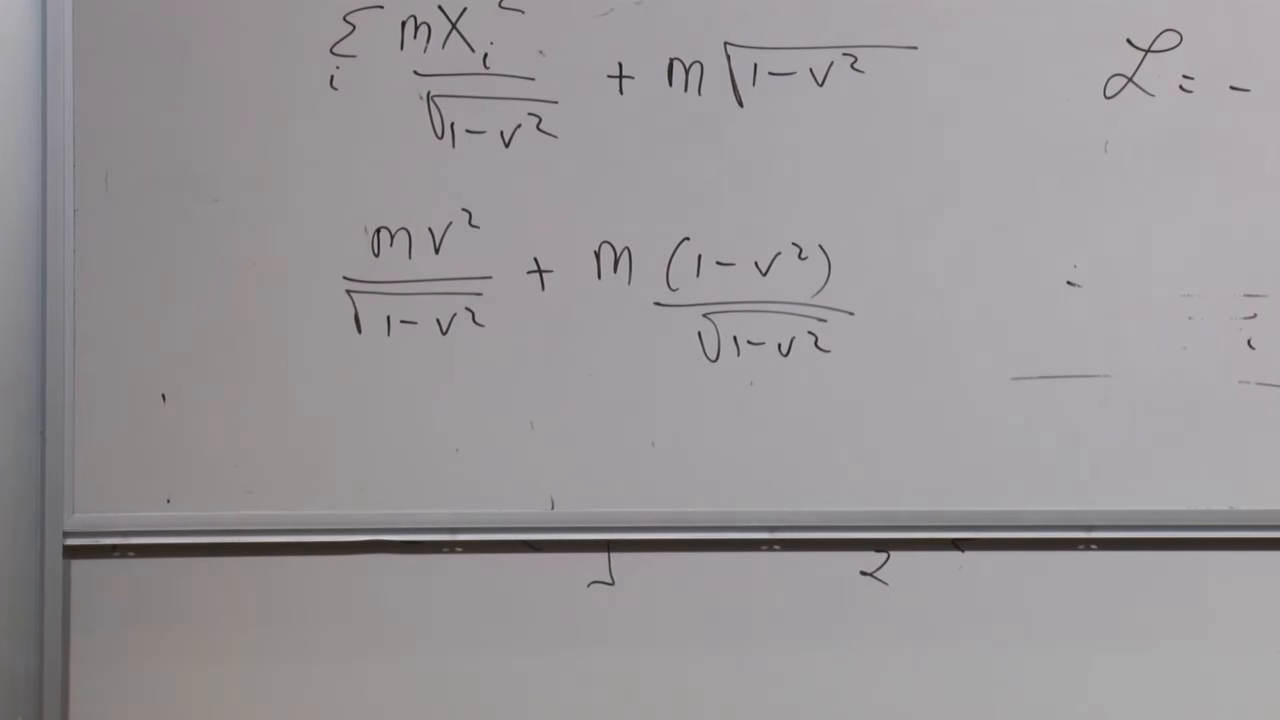
\includegraphics[width=0.90\textwidth]{lecture_03_figure_16.png}
\caption{ハミルトニアン内の2つの項は共通分母でまとめられ、\(mv^2\) の寄与は相殺する。}
\lectureframe{01:14:28}
\end{figure}

\begin{classroomqa}
\audiencequestion{式 \(H=\sum_i\dot x^i p_i-L\) は古典的なハミルトニアンの式にすぎないのか。}
\lecturerresponse{それはラグランジアンに付随する一般的なルジャンドル変換であり、特別な非相対論的仮定ではない。どの力学が得られるかは \(L\) の形が決める。ここでは相対論的な平方根のラグランジアンが \(H=m/\sqrt{1-v^2}\) を与える。\lecturetimestamp{01:15:21}}
\end{classroomqa}

不変な保存の表現は今や
\begin{equation}
\sum_{\mathrm{initial}}p^\mu
=
\sum_{\mathrm{final}}p^\mu,
\label{eq:sr3-four-momentum-conservation}
\end{equation}
であり、これはエネルギー保存と運動量の3成分すべてを1つの四元ベクトル方程式に含んでいる。

\section{静止エネルギーとニュートン極限}

自然単位では厳密なエネルギーは
\begin{equation}
E=\frac{m}{\sqrt{1-v^2}}.
\end{equation}
である。\eqref{eq:sr3-gamma-expansion} を用いると、
\begin{equation}
E
\approx
m+\frac12mv^2+\frac38mv^4+\cdots .
\label{eq:sr3-energy-natural-expansion}
\end{equation}
第2項はおなじみの運動エネルギーである。第1項は重心が静止しているときに残るエネルギーである。

\begin{figure}[htbp]
\centering
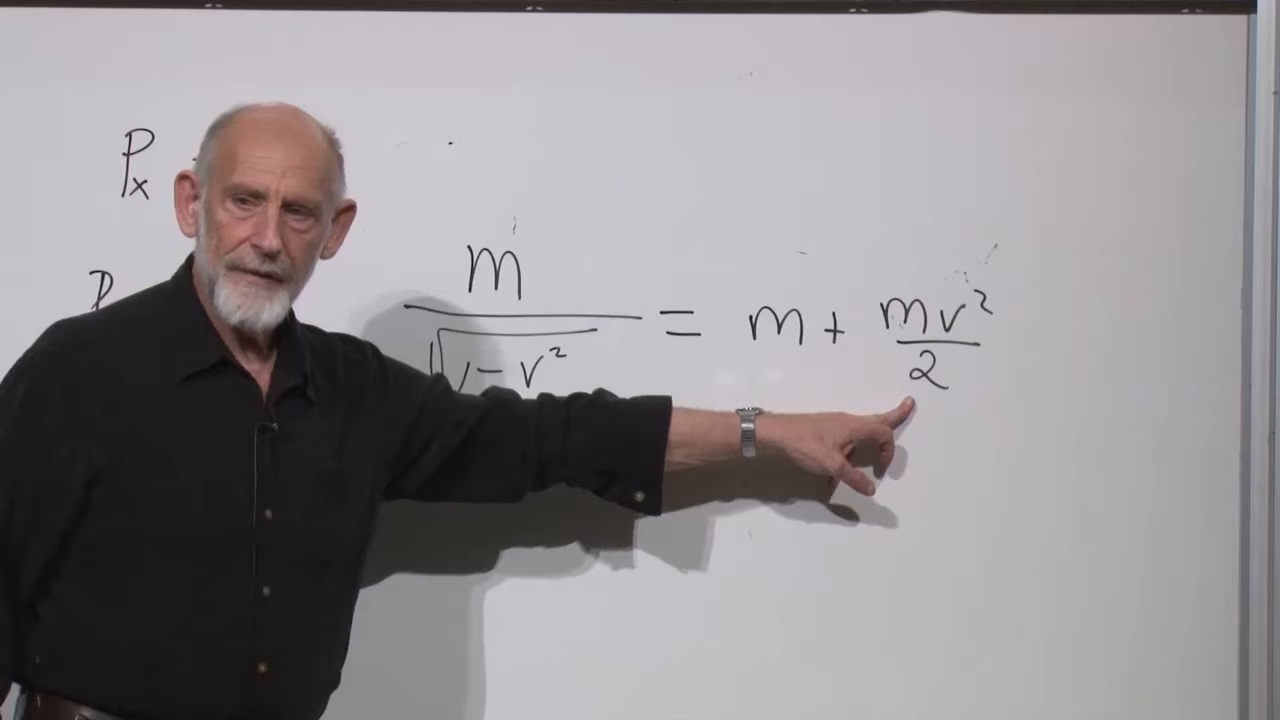
\includegraphics[width=0.90\textwidth]{lecture_03_figure_17.png}
\caption{厳密なエネルギーは単位 \(c=1\) で \(m+mv^2/2+\cdots\) と展開される。}
\lectureframe{01:18:02}
\end{figure}

厳密な表式に次元を復元する。平方根の中の比は \(v^2/c^2\) でなければならず、分子はエネルギーの単位を持たなければならない。
\begin{equation}
\boxed{
E
=
\gamma mc^2
=
\frac{mc^2}{\sqrt{1-v^2/c^2}}
}.
\label{eq:sr3-energy-exact}
\end{equation}
その低速展開は
\begin{equation}
\boxed{
E
=
mc^2+\frac12mv^2
+\frac38m\frac{v^4}{c^2}
+\cdots
}.
\label{eq:sr3-energy-dimensional-expansion}
\end{equation}
であり、静止時には
\begin{equation}
\boxed{E_{\mathrm{rest}}=mc^2}.
\label{eq:sr3-emc2}
\end{equation}
となる。

\begin{figure}[htbp]
\centering
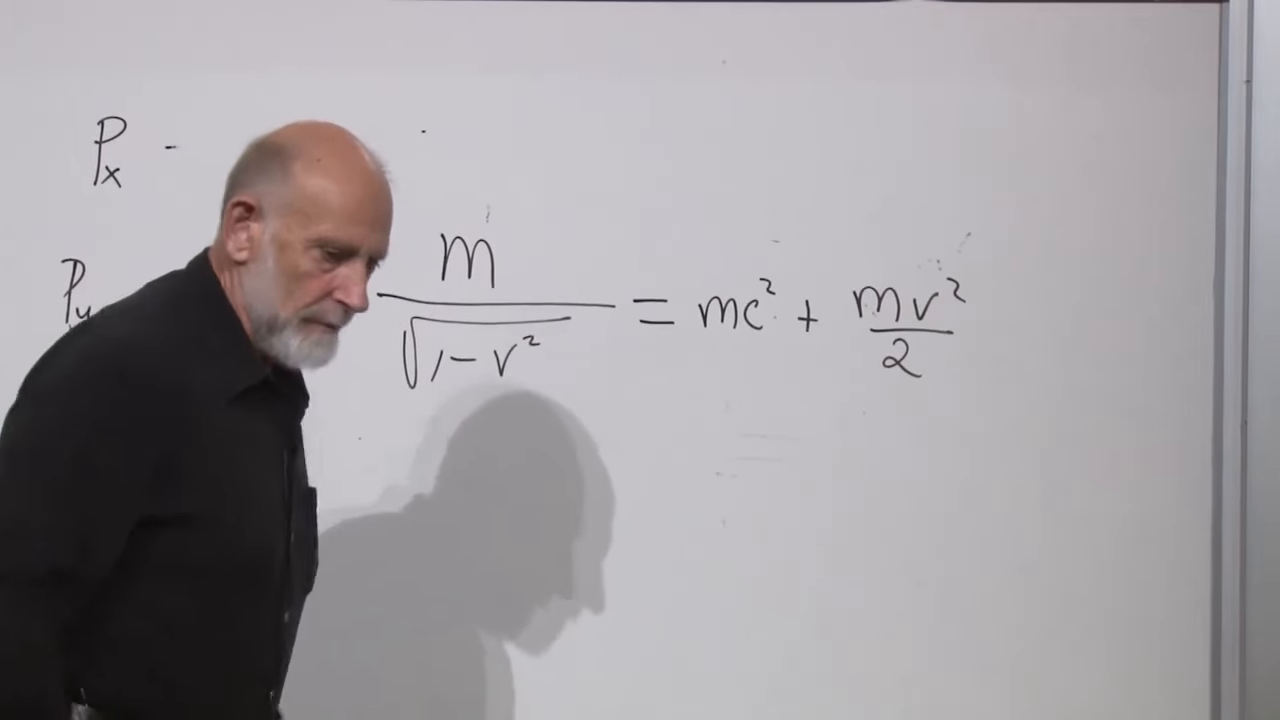
\includegraphics[width=0.90\textwidth]{lecture_03_figure_18.png}
\caption{次元の復元により、定数項は \(mc^2\) となり、それに続いてニュートン力学の運動エネルギー \(mv^2/2\) が現れる。}
\lectureframe{01:19:16}
\end{figure}

これは素粒子だけでなく、任意の閉じた物体に当てはまる。\emph{静止している}とは、重心が静止していることを意味する。物体内部の分子、原子、場は依然として運動し相互作用していてよい。それらの内部運動エネルギー、ポテンシャルエネルギー、結合エネルギーはすべて全静止エネルギーに寄与し、したがってその物体の不変質量にも寄与する。

\begin{classroomqa}
\audiencequestion{変換係数は \(c^2\) を何か任意の数で割ったものではありえないのか。}
\lecturerresponse{次元だけでは \(c\) のべきは決まるが、係数は自然単位の結果によって固定される。通常単位の式は \(c=1\) のとき \(E=m\) に帰着しなければならないので、復元された表式は静止時には係数1で \(E=mc^2\) となる。\lecturetimestamp{01:22:08}}
\end{classroomqa}

\begin{classroomqa}
\audiencequestion{二項展開の先頭の1は物理的に重要か、また高次の項は何を意味するのか。}
\lecturerresponse{はい。エネルギーの展開では先頭の1が静止エネルギー \(mc^2\) になる。次の項はニュートン力学の運動エネルギーであり、それより高次の項はすべて相対論的補正である。それらは野球のボールでは無視できるが、\(v\) が \(c\) に近づくにつれて不可欠になる。\lecturetimestamp{01:22:37}}
\end{classroomqa}

厳密なエネルギーと運動量は \(v\to c\) として発散する。
\begin{equation}
\begin{aligned}
E&=\gamma mc^2\longrightarrow\infty,\\
\vec p&=\gamma m\vec v\longrightarrow\infty
\qquad(m>0).
\end{aligned}
\end{equation}
したがって光速に到達するには無限大のエネルギーと運動量が必要となる。有限の力が有限時間作用しても有限の力積しか与えないので、質量をもつ粒子は \(c\) に近づくことはできても到達することはできない。

\begin{classroomqa}
\audiencequestion{今度は何が光速の壁を強制するのか。}
\lecturerresponse{厳密な四元運動量がそうする。質量をもつ粒子が \(c\) に近づくにつれてエネルギーと運動量の両方が発散する一方、四元運動量の保存がすべての相互作用を制約する。以前の四元速度の規格化は、同じ事柄を運動学的な形で述べたものである。\lecturetimestamp{01:24:27}}
\end{classroomqa}

\section{複合系の質量}

2つの粒子が大きさが等しく逆向きの運動量で運動しているとしよう。それらの全三次元運動量はゼロなので、すでに合成系の静止系にいることになる。その系の不変質量 \(M\) は、この系での全エネルギーによって定義される。
\begin{equation}
Mc^2=E_{\mathrm{tot}}
\qquad
(\vec P_{\mathrm{tot}}=0).
\end{equation}
より一般には、
\begin{equation}
M^2c^4
=
E_{\mathrm{tot}}^2-c^2\vec P_{\mathrm{tot}}^{\,2}.
\label{eq:sr3-composite-mass}
\end{equation}

\begin{classroomqa}
\audiencequestion{逆向きに運動する二つの粒子について、合成系の質量はそれぞれの質量の和より大きいか。}
\lecturerresponse{自由であれば、はい。重心系ではそれらの運動エネルギーが全静止エネルギーに加わるので、\(M>m_1+m_2\) となる。代わりに引力による束縛エネルギーが全体を下げることもあり、その場合は \(M<m_1+m_2\) となる。不変な定義は、全運動量が消える系における全エネルギーである。\lecturetimestamp{01:25:06}}
\end{classroomqa}

これが、複合物体の重さを測るときに内部運動と束縛を無視できない理由である。不変質量は閉じた系全体に属するものであり、構成要素の質量を単に算術的に並べたものに属するのではない。

\begin{classroomqa}
\audiencequestion{量子状態の位相において、静止エネルギーの項はどのような役割を果たすか。}
\lecturerresponse{確定したエネルギーをもつ状態は位相 \(\exp(-iEt/\hbar)\) で発展するので、静止している粒子は \(\exp(-imc^2t/\hbar)\) に寄与する。共通の全体位相は観測できないが、異なるエネルギーをもつ成分間の相対位相は観測できる。この量子的帰結はここでの古典的導出と整合するが、それを必要とするものではない。\lecturetimestamp{01:26:57}}
\end{classroomqa}

\section{エネルギー--運動量関係}

四元速度の規格化から、四元運動量の不変ノルムが直ちに得られる。\(c=1\) 単位では、
\begin{equation}
(u^0)^2-\vec u^{\,2}=1.
\end{equation}

\(m^2\) を掛け、\(p^\mu=mu^\mu\) を用いると、
\begin{equation}
\boxed{
E^2-\vec p^{\,2}=m^2
}
\qquad(c=1).
\label{eq:sr3-mass-shell-natural}
\end{equation}
同値に、
\begin{equation}
E=\sqrt{\vec p^{\,2}+m^2}.
\end{equation}

\begin{figure}[htbp]
\centering
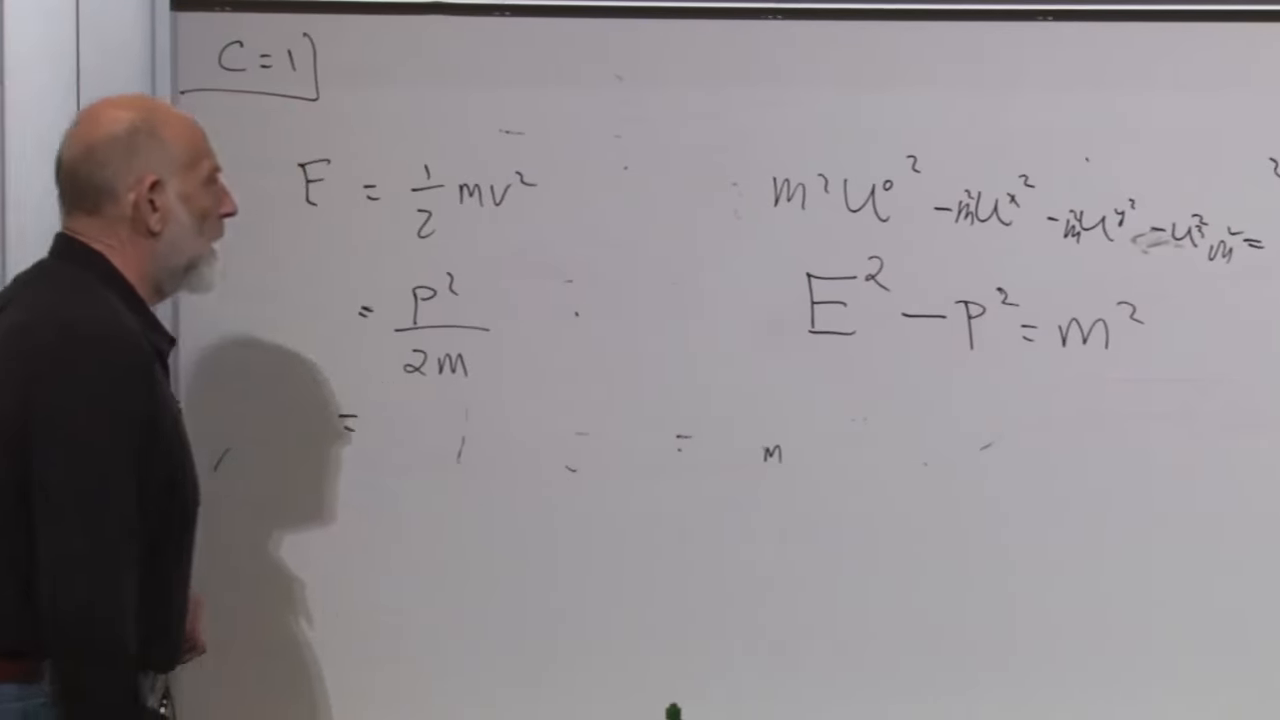
\includegraphics[width=0.90\textwidth]{lecture_03_figure_19.png}
\caption{四元速度の規格化に \(m^2\) を掛けると \(E^2-\vec p^{\,2}=m^2\) が得られる。}
\lectureframe{01:31:48}
\end{figure}

\(c\) を復元すると、
\begin{equation}
\boxed{
E^2
=
\vec p^{\,2}c^2+m^2c^4
},
\qquad
E=\sqrt{\vec p^{\,2}c^2+m^2c^4}.
\label{eq:sr3-mass-shell}
\end{equation}
この式は、速度を参照せずにエネルギーを運動量の関数として表す。これはニュートン的な関係
\begin{equation}
K=\frac{\vec p^{\,2}}{2m}.
\end{equation}
の相対論的類似である。

\begin{figure}[htbp]
\centering
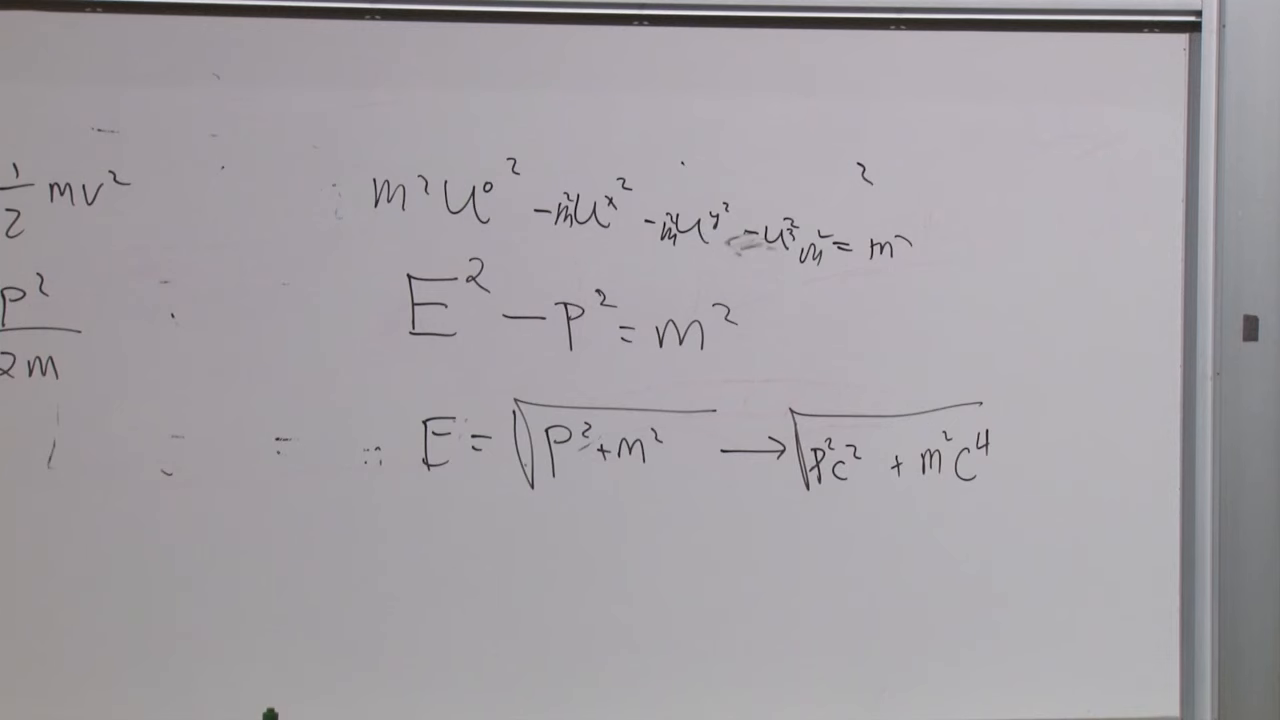
\includegraphics[width=0.90\textwidth]{lecture_03_figure_20.png}
\caption{次元を復元した質量殻関係：\(E=\sqrt{\vec p^{\,2}c^2+m^2c^4}\)。}
\lectureframe{01:32:38}
\end{figure}

\subsection{質量をもたない粒子}

速度の式 \(E=\gamma mc^2\) は、\(m=0\) かつ \(v=c\) のとき不定形 \(0/0\) になる。したがって速度は質量をもたない粒子を区別するための指標としては不適切である。真空中を自由に伝播する質量をもたない粒子はすべて \(c\) で運動するが、異なる光子は異なるエネルギーをもちうる。

エネルギー--運動量関係は滑らかな質量ゼロ極限をもつ：
\begin{equation}
m=0
\quad\Longrightarrow\quad
\boxed{E=c|\vec p|}.
\label{eq:sr3-massless-energy}
\end{equation}
これは光子に、また理想化された質量ゼロ理論では重力子に当てはまる。\(mc^2\ll E\) のときはいつでも、高度に相対論的な粒子に対する優れた近似であり、小さな非零質量をもつニュートリノも十分に高いエネルギーではこれに含まれる。

\begin{figure}[htbp]
\centering
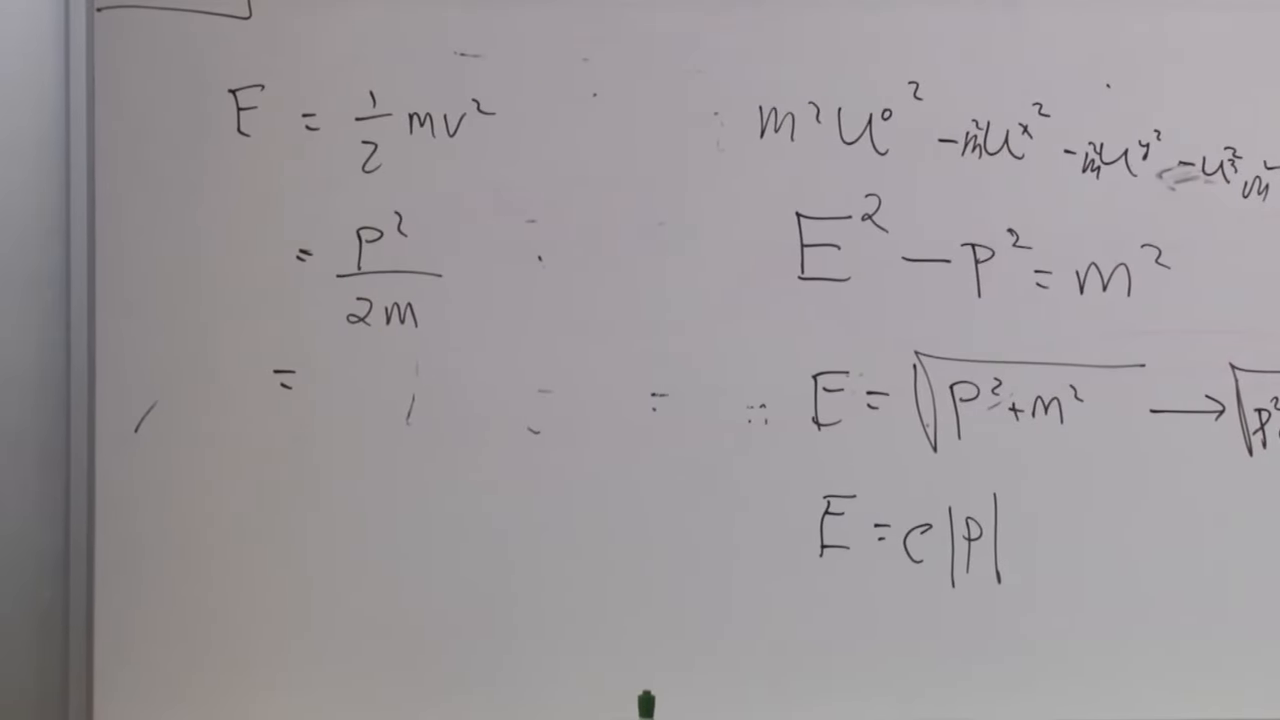
\includegraphics[width=0.90\textwidth]{lecture_03_figure_21.png}
\caption{エネルギー--運動量関係の質量ゼロ極限は \(E=c|\vec p|\) を与える。}
\lectureframe{01:33:48}
\end{figure}

\section{ポジトロニウム崩壊}

電子と陽電子の束縛状態であるポジトロニウムを考える。その不変質量は \(2m_e\) よりわずかに小さい。構成要素は正の内部運動エネルギーをもつが、それより大きな負の束縛エネルギーをもつからである。数値的には、
\begin{equation}
m_ec^2\approx0.511\ \mathrm{MeV},
\qquad
m_e\approx9.11\times10^{-31}\ \mathrm{kg},
\end{equation}
しかし運動学はその数値に依存しない。

ポジトロニウムの静止系における二光子崩壊チャネルをとる：
\begin{equation}
\mathrm{Ps}\longrightarrow\gamma+\gamma.
\end{equation}
初期の全運動量はゼロである。したがって運動量保存により、光子は等しく反対向きの運動量をもって背中合わせに放出されなければならない：
\begin{equation}
\vec p_1=\vec p,
\qquad
\vec p_2=-\vec p.
\label{eq:sr3-positronium-momentum}
\end{equation}
\(M\) をポジトロニウムの質量とすると、エネルギー保存により
\begin{equation}
Mc^2
=E_1+E_2
=c|\vec p_1|+c|\vec p_2|
=2c|\vec p|.
\end{equation}
したがって
\begin{equation}
\boxed{
|\vec p|=\frac{Mc}{2},
\qquad
E_1=E_2=\frac{Mc^2}{2}
}.
\label{eq:sr3-positronium-result}
\end{equation}

\begin{figure}[htbp]
\centering
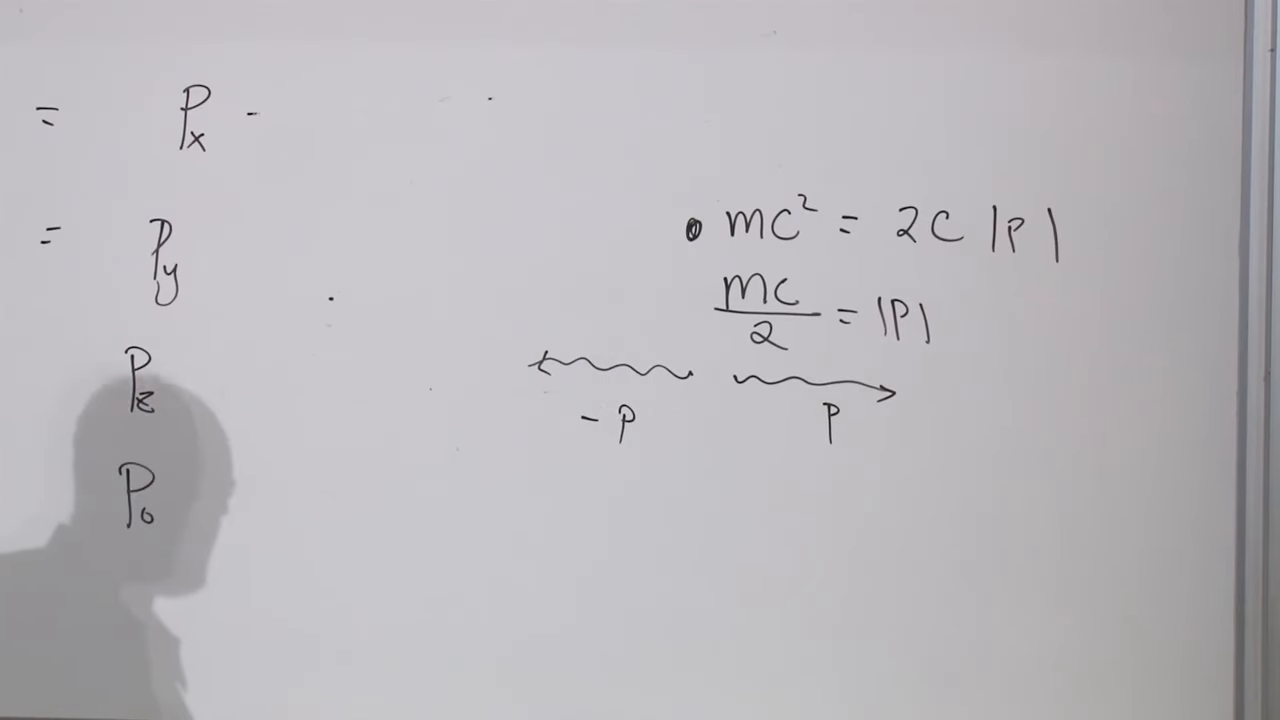
\includegraphics[width=0.90\textwidth]{lecture_03_figure_22.png}
\caption{静止したポジトロニウム状態は、等しく反対向きの運動量をもつ二つの光子に崩壊し、\(Mc^2=2c|\vec p|\) である。}
\lectureframe{01:40:55}
\end{figure}

この過程には、粒子質量の和が保存されるようなニュートン的類似は存在しない。入射状態は非零の不変質量をもつが、出ていく各光子は質量をもたない。保存されるのは全四元運動量である。蓄えられていた静止エネルギーが伝播する電磁エネルギーになったのである。量子関係 \(|\vec p|=h/\lambda\) を用いれば、同じ結果から光子の波長が定まり、対応する光子エネルギーは光学領域をはるかに超えている。

\begin{classroomqa}
\audiencequestion{崩壊において角運動量はどのように保存されるか。}
\lecturerresponse{放出される放射は、初期状態と同じ全角運動量を運ばなければならない。二光子チャネルでは、光子のヘリシティとその軌道状態が適切に結合する。より正確には、スピン一重項のパラポジトロニウムは主に二光子に崩壊し、スピン三重項のオルソポジトロニウムは主に三光子に崩壊する。許されるチャネルはすべての量子数を満たす。\lecturetimestamp{01:42:11}}
\end{classroomqa}

\begin{classroomqa}
\audiencequestion{光速で運動する粒子はなぜ質量がゼロでなければならないのか。}
\lecturerresponse{有限で非零のエネルギーに対して、因子\(\gamma\)は\(v\to c\)として発散する。不変関係\(E^2-\vec p^{\,2}c^2=m^2c^4\)は、四元運動量がヌルである粒子が\(m=0\)をもつことを示す。逆に、自由な質量ゼロの粒子はヌルの世界線をもち、\(c\)で伝播する。\lecturetimestamp{01:42:50}}
\end{classroomqa}

\begin{classroomqa}
\audiencequestion{同じ中性状態が光子の代わりに重力子へ崩壊しうるか。}
\lecturerresponse{原理的には、量子数が許すとき重力最終状態は許されるが、重力の分岐比は電磁気のそれより途方もなく小さい。運動学的な帳簿付けは依然として同じ四元運動量の保存と、各質量ゼロ量子に対する\(E=c|\vec p|\)を用いるであろう。\lecturetimestamp{01:43:20}}
\end{classroomqa}

\subsection{一つの崩壊頂点}

崩壊は局所的である。親の世界線は一つの時空事象で終わり、出ていく光子の世界線はそこで始まる。検出器との相互作用を過去へ外挿して、その共通の頂点を再構成できる。もし二つの光子が異なる事象で放出されたなら、それらの逆向き外挿されたヌル軌道は一点で交わらないであろう。

\begin{classroomqa}
\audiencequestion{二つの光子はすべての慣性系で同時に放出されなければならないのか。}
\lecturerresponse{それらは同じ時空事象で生じるのであり、同時性が慣性系に依存しうる二つの空間的に離れた事象で生じるのではない。すべてのローレンツ系は、一つの事象は一つの事象であることに同意する。量子力学は親に有限の位置不確定性を与えるので、再構成された頂点は完全に既知の古典的点ではなく分布である。\lecturetimestamp{01:44:01}}
\end{classroomqa}

\begin{classroomqa}
\audiencequestion{なぜ四元速度のノルムは1に等しいのか。}
\lecturerresponse{固有時は単位\(c=1\)で\(d\tau^2=dt^2-d\vec x^{\,2}\)により定義された。\(d\tau^2\)で割ると\((dt/d\tau)^2-(d\vec x/d\tau)^2=1\)が得られ、これはまさに\((u^0)^2-\vec u^{\,2}=1\)である。したがって規格化は固有時の定義に組み込まれている。\lecturetimestamp{01:45:38}}
\end{classroomqa}

\begin{classroomqa}
\audiencequestion{\(u^0=dt/d\tau\)はエネルギーについてより深い解釈を与えるか。}
\lecturerresponse{それは有用な恒等式\(E=mc^2\,dt/d\tau=\gamma mc^2\)を与える。すなわち、静止時には座標時と固有時の比は1であり、運動時にはそれはローレンツ因子である。その速度依存性を符号化することを超えて、この恒等式自体は別個の力学原理を付け加えるものではない。\lecturetimestamp{01:46:36}}
\end{classroomqa}

\section{保存には閉じた系が必要である}

文
\begin{equation}
\sum p^\mu_{\mathrm{initial}}
=
\sum p^\mu_{\mathrm{final}}
\end{equation}
は、エネルギーと運動量を交換するすべてを含む孤立系に適用される。現実の実験室には、漂遊電場と磁場、周囲の粒子、重力、支持体、検出器がある。それらの自由度を帳簿付けの外に置けば、部分系は小さな見かけの不均衡を示しうる。失われた四元運動量は環境へ移っているのである。

\begin{classroomqa}
\audiencequestion{二光子の運動量の和はゼロから微小量だけ異なりうるか。}
\lecturerresponse{完全な孤立系に対しては異ならない。実際の実験では、モデル化されていない場や装置の反跳がその微小な残りを運びうるので、選ばれた部分系は閉じているようには見えないかもしれない。相互作用するすべての部分を含めれば、全四元運動量は保存される。\lecturetimestamp{01:47:51}}
\end{classroomqa}

\begin{classroomqa}
\audiencequestion{不確定性原理は運動量保存を弱めるか。}
\lecturerresponse{弱めない。量子状態は位置または運動量に不確定性をもちうるし、一方をより鋭く知ることは他方の分布を広げるが、並進対称性は孤立系の全運動量の厳密な保存を依然として与える。量子不確定性は結果と分布に関するものであり、保存則の破れではない。\lecturetimestamp{01:49:19}}
\end{classroomqa}

\section{厳密なエネルギーと近似エネルギー}

厳密な式をその低速展開と混同しないことが重要である。
\begin{align}
E_{\mathrm{exact}}
&=
\frac{mc^2}{\sqrt{1-v^2/c^2}},
\label{eq:sr3-exact-repeated}\\
E_{\mathrm{slow}}
&=
mc^2+\frac12mv^2
+O\!\left(\frac{mv^4}{c^2}\right).
\label{eq:sr3-approx-repeated}
\end{align}
第一の式はすべての\(v<c\)に対して有効であり続ける。第二の式は\(v/c\ll1\)のときにのみ有用である。

\begin{classroomqa}
\audiencequestion{エネルギーの式は近似にすぎなかったのか。}
\lecturerresponse{\(E=mc^2+mv^2/2+\cdots\)が近似である。厳密な結果は\(E=mc^2/\sqrt{1-v^2/c^2}\)である。因子\(v^2/c^2\)は分母を無次元にし、一方分子\(mc^2\)はエネルギーの単位を与える。\lecturetimestamp{01:49:56}}
\end{classroomqa}

\subsection{時空の描像を再訪する}

最後の黒板のスケッチは実験の幾何学に戻る。崩壊前、静止したポジトロニウムは垂直な時間的世界線に沿う。崩壊事象でその世界線は終わり、二つのヌル光子世界線が反対の空間方向へ出発する。

\begin{figure}[htbp]
\centering
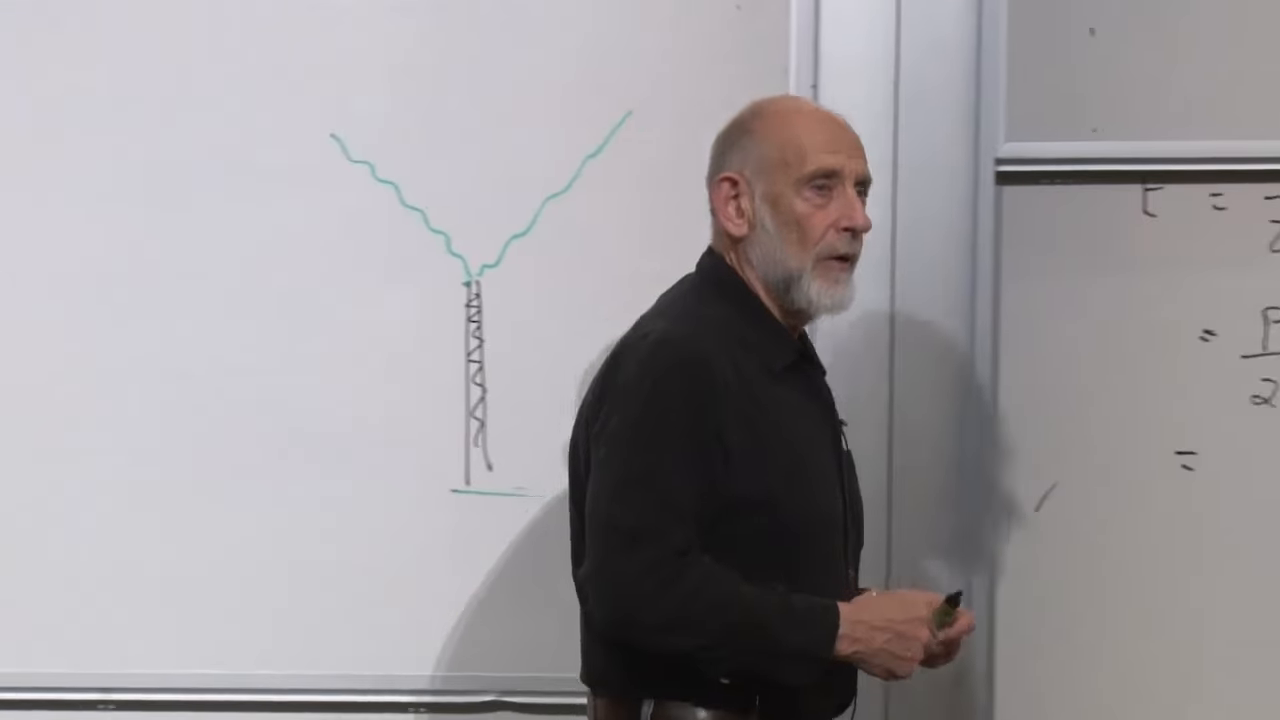
\includegraphics[width=0.90\textwidth]{lecture_03_figure_23.png}
\caption{ポジトロニウムの世界線は一つの崩壊事象で終わり、そこから二つのヌル光子世界線が現れる。}
\lectureframe{01:53:48}
\end{figure}

\begin{classroomqa}
\audiencequestion{2つの光子がどの軸に沿って現れるかを決めるものは何か。}
\lecturerresponse{非偏極状態には量子的な角度分布があり、個々の崩壊はその分布からランダムに一つの方向を選び出す。いったん一つの方向が実現すれば、運動量保存則が光子を互いに逆向きに固定するが、その軸をあらかじめ選ぶわけではない。 \lecturetimestamp{01:53:55}}
\end{classroomqa}

\section{自由な運動方程式が語ること}

不変作用は、力の法則を推測して選ばれたものではない。低速でニュートン的な自由粒子ラグランジアンを再現する、最も単純な局所ローレンツスカラーとして選ばれたのである。これを変分すると
\begin{equation}
\frac{d}{dt}\left(\frac{\partial L}{\partial\dot x^i}\right)=0,
\end{equation}
したがって
\begin{equation}
\frac{dp_i}{dt}=0.
\end{equation}
となる。固定された非零の質量に対して、これは一定の四元速度と等価である：
\begin{equation}
\frac{du^\mu}{d\tau}=0.
\end{equation}
それゆえ世界線は時空内の直線である。この一つの幾何学的な言明が、一様な速さと不変の空間的方向の両方を含んでいる。

\begin{classroomqa}
\audiencequestion{ニュートンの方程式を再現するように古典作用を選ぶのと同様に、相対論的作用に対する、よりボトムアップな正当化はあるか。}
\lecturerresponse{自由粒子に対しては、ローレンツ不変性、世界線に沿った局所性、およびニュートン的な低速極限が、全体の定数を除いて最も単純な作用を決定する。そのオイラー--ラグランジュ方程式は一定の運動量を与え、まさに無力のニュートン的結果となる。相互作用はさらなる検証を与える；後に荷電粒子が電場と磁場に結合される。 \lecturetimestamp{01:54:27}}
\end{classroomqa}

\section{二つの独立な古典極限}

非相対論的極限と量子力学の古典極限は異なる操作である。相対論的補正は比 \(v/c\) によって支配される。量子効果は \(\hbar\) に対する作用のスケール、および質量、系の大きさ、外力がどれほど滑らかに変化するかといった性質によって支配される。

\begin{classroomqa}
\audiencequestion{ニュートン力学を回復する低速極限は、量子力学が古典的になる極限と同じか。}
\lecturerresponse{いいえ。相対論的極限は \(v/c\) に関するものであり、量子から古典への極限は特徴的な作用に対する \(\hbar\) に関するものであり、しばしば大きな質量や滑らかに変化する力に対して有効になる。系は量子的だが非相対論的、相対論的だが本質的に古典的、その両方、あるいはどちらでもないことがありうる。 \lecturetimestamp{01:57:32}}
\end{classroomqa}

\begin{classroomqa}
\audiencequestion{特殊相対性理論と量子力学の間に非両立性はあるか。}
\lecturerresponse{いいえ。相対論的量子論は整合的であり、量子場の理論へと導く。有名な未解決の緊張は、重力を量子力学に取り込むことに関するものであり、特殊相対性理論と量子原理を組み合わせることではない。重力は現在の自由粒子の議論には入っていない。 \lecturetimestamp{01:59:01}}
\end{classroomqa}

今のところ、無力の結果は完全である：質量を持つ粒子はまっすぐな時間的世界線に従い、その不変質量が四元運動量のノルムを定め、エネルギーと運動量は一つの保存された対象の四つの成分である。電荷と電磁場の導入が、この自由な運動を超える次の段階となる。
